\documentclass[1p]{elsarticle_modified}
%\bibliographystyle{elsarticle-num}

%\usepackage[colorlinks]{hyperref}
%\usepackage{abbrmath_seonhwa} %\Abb, \Ascr, \Acal ,\Abf, \Afrak
\usepackage{amsfonts}
\usepackage{amssymb}
\usepackage{amsmath}
\usepackage{amsthm}
\usepackage{scalefnt}
\usepackage{amsbsy}
\usepackage{kotex}
\usepackage{caption}
\usepackage{subfig}
\usepackage{color}
\usepackage{graphicx}
\usepackage{xcolor} %% white, black, red, green, blue, cyan, magenta, yellow
\usepackage{float}
\usepackage{setspace}
\usepackage{hyperref}

\usepackage{tikz}
\usetikzlibrary{arrows}

\usepackage{multirow}
\usepackage{array} % fixed length table
\usepackage{hhline}

%%%%%%%%%%%%%%%%%%%%%
\makeatletter
\renewcommand*\env@matrix[1][\arraystretch]{%
	\edef\arraystretch{#1}%
	\hskip -\arraycolsep
	\let\@ifnextchar\new@ifnextchar
	\array{*\c@MaxMatrixCols c}}
\makeatother %https://tex.stackexchange.com/questions/14071/how-can-i-increase-the-line-spacing-in-a-matrix
%%%%%%%%%%%%%%%

\usepackage[normalem]{ulem}

\newcommand{\msout}[1]{\ifmmode\text{\sout{\ensuremath{#1}}}\else\sout{#1}\fi}
%SOURCE: \msout is \stkout macro in https://tex.stackexchange.com/questions/20609/strikeout-in-math-mode

\newcommand{\cancel}[1]{
	\ifmmode
	{\color{red}\msout{#1}}
	\else
	{\color{red}\sout{#1}}
	\fi
}

\newcommand{\add}[1]{
	{\color{blue}\uwave{#1}}
}

\newcommand{\replace}[2]{
	\ifmmode
	{\color{red}\msout{#1}}{\color{blue}\uwave{#2}}
	\else
	{\color{red}\sout{#1}}{\color{blue}\uwave{#2}}
	\fi
}

\newcommand{\Sol}{\mathcal{S}} %segment
\newcommand{\D}{D} %diagram
\newcommand{\A}{\mathcal{A}} %arc


%%%%%%%%%%%%%%%%%%%%%%%%%%%%%5 test

\def\sl{\operatorname{\textup{SL}}(2,\Cbb)}
\def\psl{\operatorname{\textup{PSL}}(2,\Cbb)}
\def\quan{\mkern 1mu \triangleright \mkern 1mu}

\theoremstyle{definition}
\newtheorem{thm}{Theorem}[section]
\newtheorem{prop}[thm]{Proposition}
\newtheorem{lem}[thm]{Lemma}
\newtheorem{ques}[thm]{Question}
\newtheorem{cor}[thm]{Corollary}
\newtheorem{defn}[thm]{Definition}
\newtheorem{exam}[thm]{Example}
\newtheorem{rmk}[thm]{Remark}
\newtheorem{alg}[thm]{Algorithm}

\newcommand{\I}{\sqrt{-1}}
\begin{document}

%\begin{frontmatter}
%
%\title{Boundary parabolic representations of knots up to 8 crossings}
%
%%% Group authors per affiliation:
%\author{Yunhi Cho} 
%\address{Department of Mathematics, University of Seoul, Seoul, Korea}
%\ead{yhcho@uos.ac.kr}
%
%
%\author{Seonhwa Kim} %\fnref{s_kim}}
%\address{Center for Geometry and Physics, Institute for Basic Science, Pohang, 37673, Korea}
%\ead{ryeona17@ibs.re.kr}
%
%\author{Hyuk Kim}
%\address{Department of Mathematical Sciences, Seoul National University, Seoul 08826, Korea}
%\ead{hyukkim@snu.ac.kr}
%
%\author{Seokbeom Yoon}
%\address{Department of Mathematical Sciences, Seoul National University, Seoul, 08826,  Korea}
%\ead{sbyoon15@snu.ac.kr}
%
%\begin{abstract}
%We find all boundary parabolic representation of knots up to 8 crossings.
%
%\end{abstract}
%\begin{keyword}
%    \MSC[2010] 57M25 
%\end{keyword}
%
%\end{frontmatter}

%\linenumbers
%\tableofcontents
%
\newcommand\colored[1]{\textcolor{white}{\rule[-0.35ex]{0.8em}{1.4ex}}\kern-0.8em\color{red} #1}%
%\newcommand\colored[1]{\textcolor{white}{ #1}\kern-2.17ex	\textcolor{white}{ #1}\kern-1.81ex	\textcolor{white}{ #1}\kern-2.15ex\color{red}#1	}

{\Large $\underline{12a_{0439}~(K12a_{0439})}$}

\setlength{\tabcolsep}{10pt}
\renewcommand{\arraystretch}{1.6}
\vspace{1cm}\begin{tabular}{m{100pt}>{\centering\arraybackslash}m{274pt}}
\multirow{5}{120pt}{
	\centering
	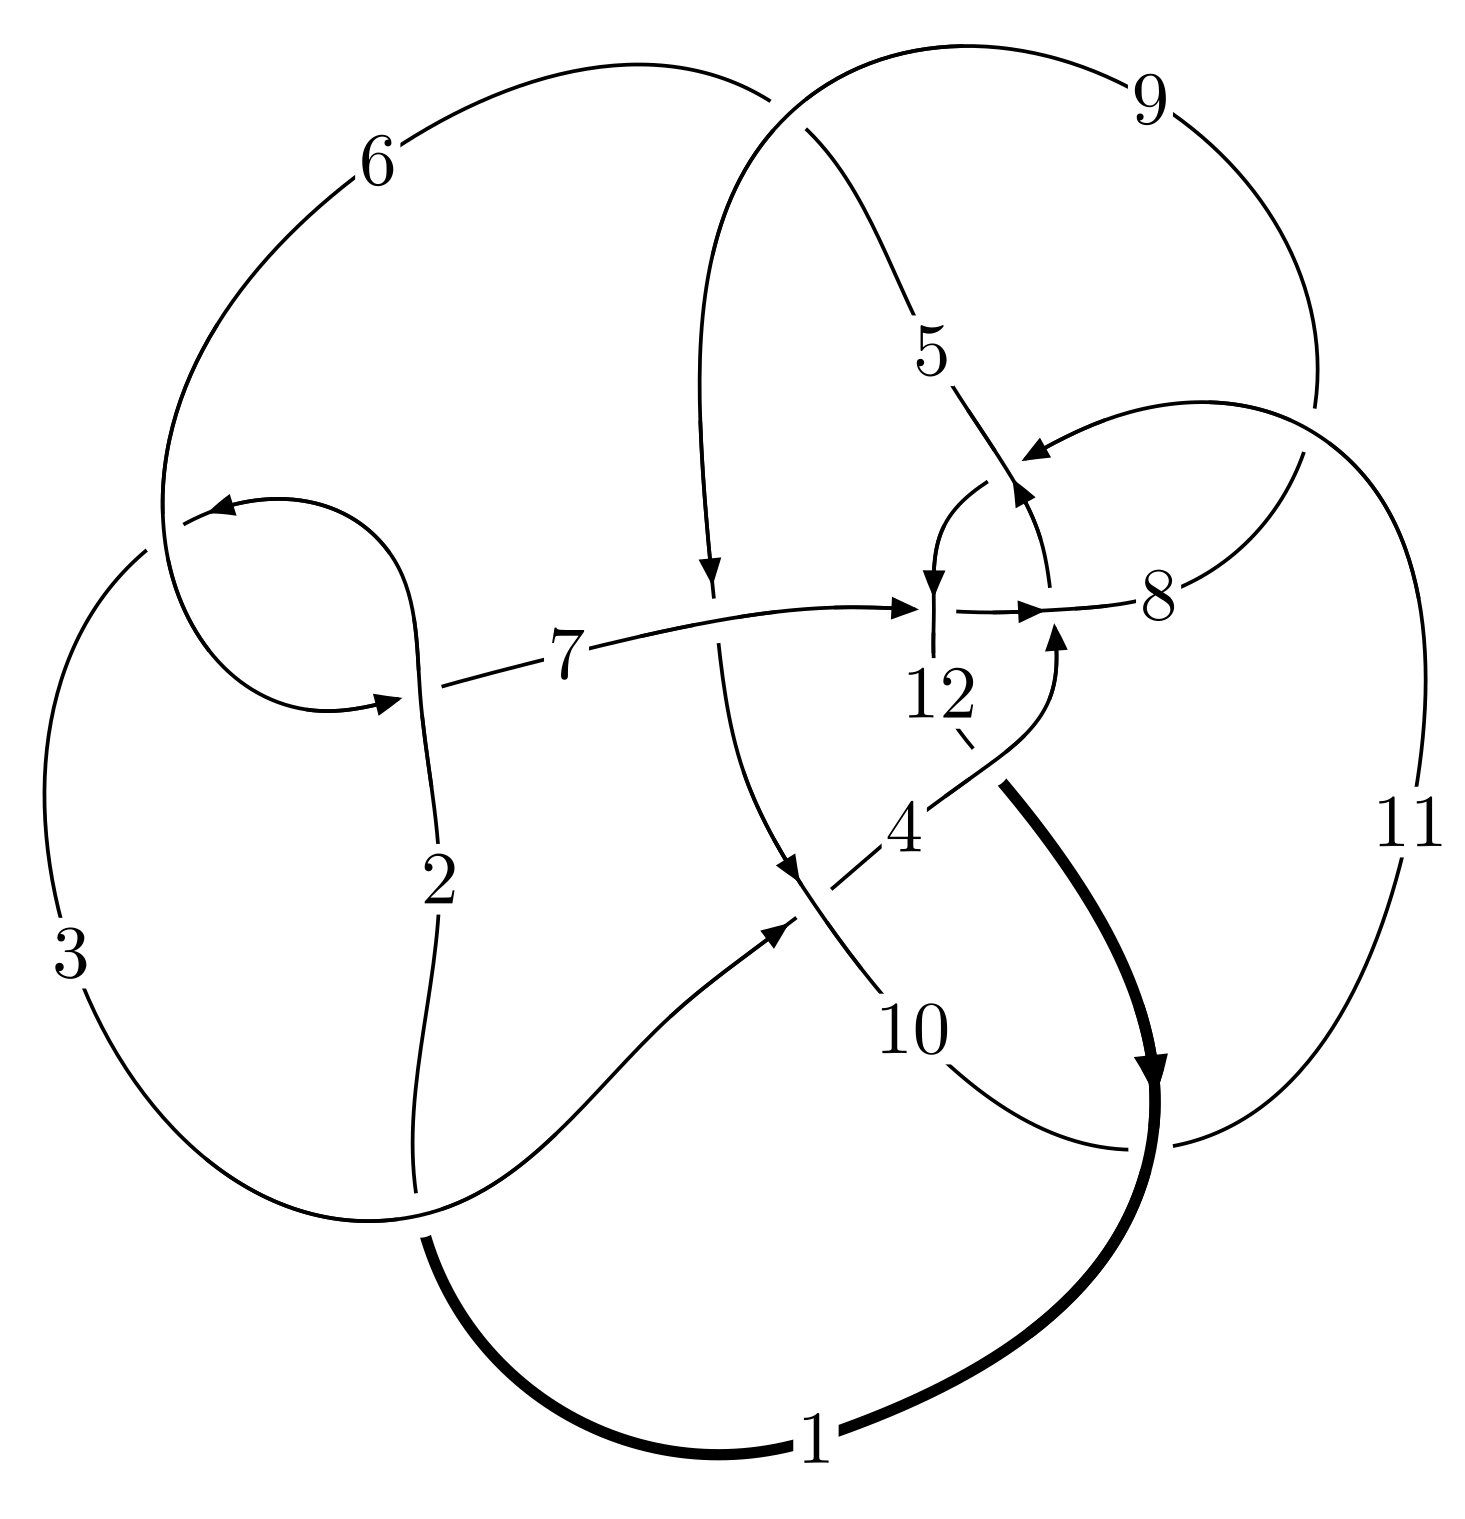
\includegraphics[width=112pt]{../../../GIT/diagram.site/Diagrams/png/1240_12a_0439.png}\\
\ \ \ A knot diagram\footnotemark}&
\allowdisplaybreaks
\textbf{Linearized knot diagam} \\
\cline{2-2}
 &
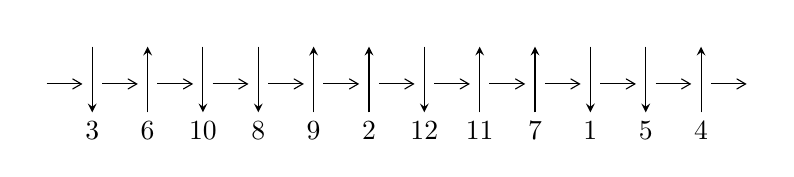
\begin{tikzpicture}[x=20pt, y=17pt]
	% nodes
	\node (C0) at (0, 0) {};
	\node (C1) at (1, 0) {};
	\node (C1U) at (1, +1) {};
	\node (C1D) at (1, -1) {3};

	\node (C2) at (2, 0) {};
	\node (C2U) at (2, +1) {};
	\node (C2D) at (2, -1) {6};

	\node (C3) at (3, 0) {};
	\node (C3U) at (3, +1) {};
	\node (C3D) at (3, -1) {10};

	\node (C4) at (4, 0) {};
	\node (C4U) at (4, +1) {};
	\node (C4D) at (4, -1) {8};

	\node (C5) at (5, 0) {};
	\node (C5U) at (5, +1) {};
	\node (C5D) at (5, -1) {9};

	\node (C6) at (6, 0) {};
	\node (C6U) at (6, +1) {};
	\node (C6D) at (6, -1) {2};

	\node (C7) at (7, 0) {};
	\node (C7U) at (7, +1) {};
	\node (C7D) at (7, -1) {12};

	\node (C8) at (8, 0) {};
	\node (C8U) at (8, +1) {};
	\node (C8D) at (8, -1) {11};

	\node (C9) at (9, 0) {};
	\node (C9U) at (9, +1) {};
	\node (C9D) at (9, -1) {7};

	\node (C10) at (10, 0) {};
	\node (C10U) at (10, +1) {};
	\node (C10D) at (10, -1) {1};

	\node (C11) at (11, 0) {};
	\node (C11U) at (11, +1) {};
	\node (C11D) at (11, -1) {5};

	\node (C12) at (12, 0) {};
	\node (C12U) at (12, +1) {};
	\node (C12D) at (12, -1) {4};
	\node (C13) at (13, 0) {};

	% arrows
	\draw[->,>={angle 60}]
	(C0) edge (C1) (C1) edge (C2) (C2) edge (C3) (C3) edge (C4) (C4) edge (C5) (C5) edge (C6) (C6) edge (C7) (C7) edge (C8) (C8) edge (C9) (C9) edge (C10) (C10) edge (C11) (C11) edge (C12) (C12) edge (C13) ;	\draw[->,>=stealth]
	(C1U) edge (C1D) (C2D) edge (C2U) (C3U) edge (C3D) (C4U) edge (C4D) (C5D) edge (C5U) (C6D) edge (C6U) (C7U) edge (C7D) (C8D) edge (C8U) (C9D) edge (C9U) (C10U) edge (C10D) (C11U) edge (C11D) (C12D) edge (C12U) ;
	\end{tikzpicture} \\
\hhline{~~} \\& 
\textbf{Solving Sequence} \\ \cline{2-2} 
 &
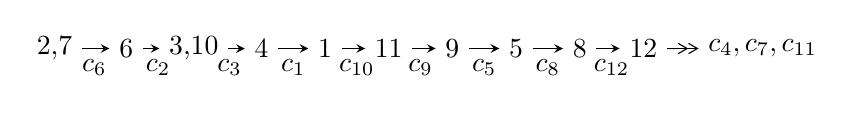
\begin{tikzpicture}[x=23pt, y=7pt]
	% node
	\node (A0) at (-1/8, 0) {2,7};
	\node (A1) at (1, 0) {6};
	\node (A2) at (33/16, 0) {3,10};
	\node (A3) at (25/8, 0) {4};
	\node (A4) at (33/8, 0) {1};
	\node (A5) at (41/8, 0) {11};
	\node (A6) at (49/8, 0) {9};
	\node (A7) at (57/8, 0) {5};
	\node (A8) at (65/8, 0) {8};
	\node (A9) at (73/8, 0) {12};
	\node (C1) at (1/2, -1) {$c_{6}$};
	\node (C2) at (3/2, -1) {$c_{2}$};
	\node (C3) at (21/8, -1) {$c_{3}$};
	\node (C4) at (29/8, -1) {$c_{1}$};
	\node (C5) at (37/8, -1) {$c_{10}$};
	\node (C6) at (45/8, -1) {$c_{9}$};
	\node (C7) at (53/8, -1) {$c_{5}$};
	\node (C8) at (61/8, -1) {$c_{8}$};
	\node (C9) at (69/8, -1) {$c_{12}$};
	\node (A10) at (11, 0) {$c_{4},c_{7},c_{11}$};

	% edge
	\draw[->,>=stealth]	
	(A0) edge (A1) (A1) edge (A2) (A2) edge (A3) (A3) edge (A4) (A4) edge (A5) (A5) edge (A6) (A6) edge (A7) (A7) edge (A8) (A8) edge (A9) ;
	\draw[->>,>={angle 60}]	
	(A9) edge (A10);
\end{tikzpicture} \\ 

\end{tabular} \\

\footnotetext{
The image of knot diagram is generated by the software ``\textbf{Draw programme}" developed by Andrew Bartholomew(\url{http://www.layer8.co.uk/maths/draw/index.htm\#Running-draw}), where we modified some parts for our purpose(\url{https://github.com/CATsTAILs/LinksPainter}).
}\phantom \\ \newline 
\centering \textbf{Ideals for irreducible components\footnotemark of $X_{\text{par}}$} 
 
\begin{align*}
I^u_{1}&=\langle 
-5.09741\times10^{706} u^{198}-3.08612\times10^{706} u^{197}+\cdots+2.09580\times10^{706} b+1.26886\times10^{709},\\
\phantom{I^u_{1}}&\phantom{= \langle  }-1.78590\times10^{709} u^{198}+9.32188\times10^{708} u^{197}+\cdots+2.91316\times10^{708} a+1.59296\times10^{711},\\
\phantom{I^u_{1}}&\phantom{= \langle  }u^{199}+40 u^{197}+\cdots-886 u-139\rangle \\
I^u_{2}&=\langle 
9.05599\times10^{16} u^{38}-1.21944\times10^{17} u^{37}+\cdots+1.56396\times10^{17} b-8.41549\times10^{16},\\
\phantom{I^u_{2}}&\phantom{= \langle  }1.35450\times10^{17} u^{38}+1.15254\times10^{17} u^{37}+\cdots+1.56396\times10^{17} a-4.55146\times10^{17},\;u^{39}+u^{38}+\cdots-2 u+1\rangle \\
\\
\end{align*}
\raggedright * 2 irreducible components of $\dim_{\mathbb{C}}=0$, with total 238 representations.\\
\footnotetext{All coefficients of polynomials are rational numbers. But the coefficients are sometimes approximated in decimal forms when there is not enough margin.}
\newpage
\renewcommand{\arraystretch}{1}
\centering \section*{I. $I^u_{1}= \langle -5.10\times10^{706} u^{198}-3.09\times10^{706} u^{197}+\cdots+2.10\times10^{706} b+1.27\times10^{709},\;-1.79\times10^{709} u^{198}+9.32\times10^{708} u^{197}+\cdots+2.91\times10^{708} a+1.59\times10^{711},\;u^{199}+40 u^{197}+\cdots-886 u-139 \rangle$}
\flushleft \textbf{(i) Arc colorings}\\
\begin{tabular}{m{7pt} m{180pt} m{7pt} m{180pt} }
\flushright $a_{2}=$&$\begin{pmatrix}0\\u\end{pmatrix}$ \\
\flushright $a_{7}=$&$\begin{pmatrix}1\\0\end{pmatrix}$ \\
\flushright $a_{6}=$&$\begin{pmatrix}1\\u^2\end{pmatrix}$ \\
\flushright $a_{3}=$&$\begin{pmatrix}u\\u^3+u\end{pmatrix}$ \\
\flushright $a_{10}=$&$\begin{pmatrix}6.13044 u^{198}-3.19992 u^{197}+\cdots-3739.45 u-546.816\\2.43220 u^{198}+1.47253 u^{197}+\cdots-3493.24 u-605.430\end{pmatrix}$ \\
\flushright $a_{4}=$&$\begin{pmatrix}4.17955 u^{198}+0.616113 u^{197}+\cdots-4122.45 u-662.313\\1.45668 u^{198}-2.78421 u^{197}+\cdots+594.418 u+149.180\end{pmatrix}$ \\
\flushright $a_{1}=$&$\begin{pmatrix}u^3\\u^5+u^3+u\end{pmatrix}$ \\
\flushright $a_{11}=$&$\begin{pmatrix}4.09110 u^{198}-3.67876 u^{197}+\cdots-1327.70 u-134.756\\1.44768 u^{198}+1.44308 u^{197}+\cdots-2495.03 u-443.280\end{pmatrix}$ \\
\flushright $a_{9}=$&$\begin{pmatrix}3.69824 u^{198}-4.67245 u^{197}+\cdots-246.204 u+58.6142\\2.43220 u^{198}+1.47253 u^{197}+\cdots-3493.24 u-605.430\end{pmatrix}$ \\
\flushright $a_{5}=$&$\begin{pmatrix}-4.00690 u^{198}-2.71923 u^{197}+\cdots+5508.41 u+933.641\\-0.755236 u^{198}+1.30418 u^{197}+\cdots-297.396 u-75.4139\end{pmatrix}$ \\
\flushright $a_{8}=$&$\begin{pmatrix}0.736592 u^{198}-2.09312 u^{197}+\cdots+505.805 u+125.305\\-1.14676 u^{198}+0.921419 u^{197}+\cdots+564.378 u+70.9771\end{pmatrix}$ \\
\flushright $a_{12}=$&$\begin{pmatrix}-15.2221 u^{198}+2.57203 u^{197}+\cdots+12340.0 u+1899.53\\2.28124 u^{198}-0.641223 u^{197}+\cdots-1770.10 u-274.405\end{pmatrix}$\\&\end{tabular}
\flushleft \textbf{(ii) Obstruction class $= -1$}\\~\\
\flushleft \textbf{(iii) Cusp Shapes $= 21.1479 u^{198}-52.4779 u^{197}+\cdots+20179.0 u+4338.51$}\\~\\
\newpage\renewcommand{\arraystretch}{1}
\flushleft \textbf{(iv) u-Polynomials at the component}\newline \\
\begin{tabular}{m{50pt}|m{274pt}}
Crossings & \hspace{64pt}u-Polynomials at each crossing \\
\hline $$\begin{aligned}c_{1}\end{aligned}$$&$\begin{aligned}
&u^{199}+80 u^{198}+\cdots-682010 u-19321
\end{aligned}$\\
\hline $$\begin{aligned}c_{2},c_{6}\end{aligned}$$&$\begin{aligned}
&u^{199}+40 u^{197}+\cdots-886 u+139
\end{aligned}$\\
\hline $$\begin{aligned}c_{3}\end{aligned}$$&$\begin{aligned}
&u^{199}+4 u^{197}+\cdots-15 u+2
\end{aligned}$\\
\hline $$\begin{aligned}c_{4}\end{aligned}$$&$\begin{aligned}
&u^{199}+4 u^{198}+\cdots-43 u+7
\end{aligned}$\\
\hline $$\begin{aligned}c_{5}\end{aligned}$$&$\begin{aligned}
&u^{199}+u^{198}+\cdots+3083941 u-3270107
\end{aligned}$\\
\hline $$\begin{aligned}c_{7}\end{aligned}$$&$\begin{aligned}
&u^{199}-4 u^{198}+\cdots-48 u+1
\end{aligned}$\\
\hline $$\begin{aligned}c_{8}\end{aligned}$$&$\begin{aligned}
&u^{199}-13 u^{198}+\cdots+67 u+1
\end{aligned}$\\
\hline $$\begin{aligned}c_{9}\end{aligned}$$&$\begin{aligned}
&u^{199}-5 u^{198}+\cdots-35977 u-38728
\end{aligned}$\\
\hline $$\begin{aligned}c_{10}\end{aligned}$$&$\begin{aligned}
&u^{199}+2 u^{198}+\cdots-73602 u+7609
\end{aligned}$\\
\hline $$\begin{aligned}c_{11}\end{aligned}$$&$\begin{aligned}
&u^{199}+2 u^{198}+\cdots-81 u+4
\end{aligned}$\\
\hline $$\begin{aligned}c_{12}\end{aligned}$$&$\begin{aligned}
&u^{199}+14 u^{198}+\cdots+7 u-1
\end{aligned}$\\
\hline
\end{tabular}\\~\\
\newpage\renewcommand{\arraystretch}{1}
\flushleft \textbf{(v) Riley Polynomials at the component}\newline \\
\begin{tabular}{m{50pt}|m{274pt}}
Crossings & \hspace{64pt}Riley Polynomials at each crossing \\
\hline $$\begin{aligned}c_{1}\end{aligned}$$&$\begin{aligned}
&y^{199}+84 y^{198}+\cdots-5691751490 y-373301041
\end{aligned}$\\
\hline $$\begin{aligned}c_{2},c_{6}\end{aligned}$$&$\begin{aligned}
&y^{199}+80 y^{198}+\cdots-682010 y-19321
\end{aligned}$\\
\hline $$\begin{aligned}c_{3}\end{aligned}$$&$\begin{aligned}
&y^{199}+8 y^{198}+\cdots+809 y-4
\end{aligned}$\\
\hline $$\begin{aligned}c_{4}\end{aligned}$$&$\begin{aligned}
&y^{199}-30 y^{198}+\cdots-41 y-49
\end{aligned}$\\
\hline $$\begin{aligned}c_{5}\end{aligned}$$&$\begin{aligned}
&y^{199}-73 y^{198}+\cdots+323847798103351 y-10693599791449
\end{aligned}$\\
\hline $$\begin{aligned}c_{7}\end{aligned}$$&$\begin{aligned}
&y^{199}-12 y^{198}+\cdots+64 y-1
\end{aligned}$\\
\hline $$\begin{aligned}c_{8}\end{aligned}$$&$\begin{aligned}
&y^{199}-21 y^{198}+\cdots+205 y-1
\end{aligned}$\\
\hline $$\begin{aligned}c_{9}\end{aligned}$$&$\begin{aligned}
&y^{199}-41 y^{198}+\cdots+110633557809 y-1499857984
\end{aligned}$\\
\hline $$\begin{aligned}c_{10}\end{aligned}$$&$\begin{aligned}
&y^{199}+8 y^{198}+\cdots-4561096888 y-57896881
\end{aligned}$\\
\hline $$\begin{aligned}c_{11}\end{aligned}$$&$\begin{aligned}
&y^{199}+6 y^{198}+\cdots-1495 y-16
\end{aligned}$\\
\hline $$\begin{aligned}c_{12}\end{aligned}$$&$\begin{aligned}
&y^{199}+44 y^{198}+\cdots-2003 y-1
\end{aligned}$\\
\hline
\end{tabular}\\~\\
\newpage\flushleft \textbf{(vi) Complex Volumes and Cusp Shapes}
$$\begin{array}{c|c|c}  
\text{Solutions to }I^u_{1}& \I (\text{vol} + \sqrt{-1}CS) & \text{Cusp shape}\\
 \hline 
\begin{aligned}
u &= -0.587023 + 0.809948 I \\
a &= -1.58919 - 1.33971 I \\
b &= -1.68634 - 0.71778 I\end{aligned}
 & \phantom{-}3.11712 - 1.71695 I & \phantom{-0.000000 } 0 \\ \hline\begin{aligned}
u &= -0.587023 - 0.809948 I \\
a &= -1.58919 + 1.33971 I \\
b &= -1.68634 + 0.71778 I\end{aligned}
 & \phantom{-}3.11712 + 1.71695 I & \phantom{-0.000000 } 0 \\ \hline\begin{aligned}
u &= \phantom{-}0.498494 + 0.869106 I \\
a &= \phantom{-}1.51301 - 0.12512 I \\
b &= -0.06660 + 1.91633 I\end{aligned}
 & -2.46657 - 1.63655 I & \phantom{-0.000000 } 0 \\ \hline\begin{aligned}
u &= \phantom{-}0.498494 - 0.869106 I \\
a &= \phantom{-}1.51301 + 0.12512 I \\
b &= -0.06660 - 1.91633 I\end{aligned}
 & -2.46657 + 1.63655 I & \phantom{-0.000000 } 0 \\ \hline\begin{aligned}
u &= \phantom{-}0.846999 + 0.545832 I \\
a &= -1.30555 + 0.81965 I \\
b &= -1.58559 + 0.36312 I\end{aligned}
 & \phantom{-}4.92626 - 3.40647 I & \phantom{-0.000000 } 0 \\ \hline\begin{aligned}
u &= \phantom{-}0.846999 - 0.545832 I \\
a &= -1.30555 - 0.81965 I \\
b &= -1.58559 - 0.36312 I\end{aligned}
 & \phantom{-}4.92626 + 3.40647 I & \phantom{-0.000000 } 0 \\ \hline\begin{aligned}
u &= \phantom{-}0.460856 + 0.898481 I \\
a &= -2.31383 - 0.07866 I \\
b &= -0.58153 - 1.29075 I\end{aligned}
 & -2.56759 + 5.97714 I & \phantom{-0.000000 } 0 \\ \hline\begin{aligned}
u &= \phantom{-}0.460856 - 0.898481 I \\
a &= -2.31383 + 0.07866 I \\
b &= -0.58153 + 1.29075 I\end{aligned}
 & -2.56759 - 5.97714 I & \phantom{-0.000000 } 0 \\ \hline\begin{aligned}
u &= \phantom{-}0.658313 + 0.738587 I \\
a &= \phantom{-}1.086630 + 0.630093 I \\
b &= -0.12798 + 1.62661 I\end{aligned}
 & \phantom{-}3.69763 - 1.62018 I & \phantom{-0.000000 } 0 \\ \hline\begin{aligned}
u &= \phantom{-}0.658313 - 0.738587 I \\
a &= \phantom{-}1.086630 - 0.630093 I \\
b &= -0.12798 - 1.62661 I\end{aligned}
 & \phantom{-}3.69763 + 1.62018 I & \phantom{-0.000000 } 0\\
 \hline 
 \end{array}$$\newpage$$\begin{array}{c|c|c}  
\text{Solutions to }I^u_{1}& \I (\text{vol} + \sqrt{-1}CS) & \text{Cusp shape}\\
 \hline 
\begin{aligned}
u &= \phantom{-}0.496193 + 0.885382 I \\
a &= -0.595402 - 0.418175 I \\
b &= \phantom{-}0.42150 - 1.71955 I\end{aligned}
 & -2.51095 + 5.65371 I & \phantom{-0.000000 } 0 \\ \hline\begin{aligned}
u &= \phantom{-}0.496193 - 0.885382 I \\
a &= -0.595402 + 0.418175 I \\
b &= \phantom{-}0.42150 + 1.71955 I\end{aligned}
 & -2.51095 - 5.65371 I & \phantom{-0.000000 } 0 \\ \hline\begin{aligned}
u &= -0.620370 + 0.810880 I \\
a &= \phantom{-}2.59463 + 1.02657 I \\
b &= \phantom{-}1.95146 - 1.71839 I\end{aligned}
 & \phantom{-}1.92152 + 5.87036 I & \phantom{-0.000000 } 0 \\ \hline\begin{aligned}
u &= -0.620370 - 0.810880 I \\
a &= \phantom{-}2.59463 - 1.02657 I \\
b &= \phantom{-}1.95146 + 1.71839 I\end{aligned}
 & \phantom{-}1.92152 - 5.87036 I & \phantom{-0.000000 } 0 \\ \hline\begin{aligned}
u &= -0.603665 + 0.824516 I \\
a &= \phantom{-}1.53484 - 0.22769 I \\
b &= \phantom{-}0.568051 + 0.304538 I\end{aligned}
 & \phantom{-}0.829209 - 0.961634 I & \phantom{-0.000000 } 0 \\ \hline\begin{aligned}
u &= -0.603665 - 0.824516 I \\
a &= \phantom{-}1.53484 + 0.22769 I \\
b &= \phantom{-}0.568051 - 0.304538 I\end{aligned}
 & \phantom{-}0.829209 + 0.961634 I & \phantom{-0.000000 } 0 \\ \hline\begin{aligned}
u &= -0.562447 + 0.796277 I \\
a &= -0.92089 - 1.49319 I \\
b &= -0.297810 + 0.803227 I\end{aligned}
 & \phantom{-}0.711468 + 0.652990 I & \phantom{-0.000000 } 0 \\ \hline\begin{aligned}
u &= -0.562447 - 0.796277 I \\
a &= -0.92089 + 1.49319 I \\
b &= -0.297810 - 0.803227 I\end{aligned}
 & \phantom{-}0.711468 - 0.652990 I & \phantom{-0.000000 } 0 \\ \hline\begin{aligned}
u &= \phantom{-}0.632151 + 0.738294 I \\
a &= \phantom{-}1.58039 + 0.00282 I \\
b &= \phantom{-}1.087880 - 0.551446 I\end{aligned}
 & \phantom{-}2.49967 - 7.27688 I & \phantom{-0.000000 } 0 \\ \hline\begin{aligned}
u &= \phantom{-}0.632151 - 0.738294 I \\
a &= \phantom{-}1.58039 - 0.00282 I \\
b &= \phantom{-}1.087880 + 0.551446 I\end{aligned}
 & \phantom{-}2.49967 + 7.27688 I & \phantom{-0.000000 } 0\\
 \hline 
 \end{array}$$\newpage$$\begin{array}{c|c|c}  
\text{Solutions to }I^u_{1}& \I (\text{vol} + \sqrt{-1}CS) & \text{Cusp shape}\\
 \hline 
\begin{aligned}
u &= \phantom{-}0.149466 + 1.023060 I \\
a &= -0.028958 + 0.371393 I \\
b &= -0.389972 - 1.267390 I\end{aligned}
 & -3.55097 + 5.84813 I & \phantom{-0.000000 } 0 \\ \hline\begin{aligned}
u &= \phantom{-}0.149466 - 1.023060 I \\
a &= -0.028958 - 0.371393 I \\
b &= -0.389972 + 1.267390 I\end{aligned}
 & -3.55097 - 5.84813 I & \phantom{-0.000000 } 0 \\ \hline\begin{aligned}
u &= \phantom{-}0.642200 + 0.719775 I \\
a &= -0.344194 + 1.050210 I \\
b &= -1.12875 + 1.12848 I\end{aligned}
 & \phantom{-}3.38444 - 1.25481 I & \phantom{-0.000000 } 0 \\ \hline\begin{aligned}
u &= \phantom{-}0.642200 - 0.719775 I \\
a &= -0.344194 - 1.050210 I \\
b &= -1.12875 - 1.12848 I\end{aligned}
 & \phantom{-}3.38444 + 1.25481 I & \phantom{-0.000000 } 0 \\ \hline\begin{aligned}
u &= \phantom{-}0.343751 + 0.893683 I \\
a &= \phantom{-}1.40662 - 0.56403 I \\
b &= \phantom{-}0.939545 + 0.438048 I\end{aligned}
 & -3.08732 - 0.74941 I & \phantom{-0.000000 } 0 \\ \hline\begin{aligned}
u &= \phantom{-}0.343751 - 0.893683 I \\
a &= \phantom{-}1.40662 + 0.56403 I \\
b &= \phantom{-}0.939545 - 0.438048 I\end{aligned}
 & -3.08732 + 0.74941 I & \phantom{-0.000000 } 0 \\ \hline\begin{aligned}
u &= -0.590646 + 0.860453 I \\
a &= \phantom{-}1.66359 + 1.64155 I \\
b &= \phantom{-}0.346971 - 0.404625 I\end{aligned}
 & \phantom{-}0.72523 - 3.77033 I & \phantom{-0.000000 } 0 \\ \hline\begin{aligned}
u &= -0.590646 - 0.860453 I \\
a &= \phantom{-}1.66359 - 1.64155 I \\
b &= \phantom{-}0.346971 + 0.404625 I\end{aligned}
 & \phantom{-}0.72523 + 3.77033 I & \phantom{-0.000000 } 0 \\ \hline\begin{aligned}
u &= -0.061841 + 1.043210 I \\
a &= \phantom{-}0.758876 + 0.278900 I \\
b &= -0.572943 + 0.413690 I\end{aligned}
 & -1.22030 - 2.21742 I & \phantom{-0.000000 } 0 \\ \hline\begin{aligned}
u &= -0.061841 - 1.043210 I \\
a &= \phantom{-}0.758876 - 0.278900 I \\
b &= -0.572943 - 0.413690 I\end{aligned}
 & -1.22030 + 2.21742 I & \phantom{-0.000000 } 0\\
 \hline 
 \end{array}$$\newpage$$\begin{array}{c|c|c}  
\text{Solutions to }I^u_{1}& \I (\text{vol} + \sqrt{-1}CS) & \text{Cusp shape}\\
 \hline 
\begin{aligned}
u &= \phantom{-}0.909196 + 0.515496 I \\
a &= \phantom{-}1.055940 - 0.828951 I \\
b &= \phantom{-}1.061930 - 0.732069 I\end{aligned}
 & \phantom{-}1.33611 - 7.53363 I & \phantom{-0.000000 } 0 \\ \hline\begin{aligned}
u &= \phantom{-}0.909196 - 0.515496 I \\
a &= \phantom{-}1.055940 + 0.828951 I \\
b &= \phantom{-}1.061930 + 0.732069 I\end{aligned}
 & \phantom{-}1.33611 + 7.53363 I & \phantom{-0.000000 } 0 \\ \hline\begin{aligned}
u &= \phantom{-}0.903016 + 0.546950 I \\
a &= -0.93396 + 1.12986 I \\
b &= -1.22277 + 1.21905 I\end{aligned}
 & \phantom{-}3.79969 - 7.43778 I & \phantom{-0.000000 } 0 \\ \hline\begin{aligned}
u &= \phantom{-}0.903016 - 0.546950 I \\
a &= -0.93396 - 1.12986 I \\
b &= -1.22277 - 1.21905 I\end{aligned}
 & \phantom{-}3.79969 + 7.43778 I & \phantom{-0.000000 } 0 \\ \hline\begin{aligned}
u &= -0.528333 + 0.781637 I \\
a &= -1.29996 + 1.74911 I \\
b &= -0.936537 - 0.153818 I\end{aligned}
 & \phantom{-}1.79008 - 1.57341 I & \phantom{-0.000000 } 0 \\ \hline\begin{aligned}
u &= -0.528333 - 0.781637 I \\
a &= -1.29996 - 1.74911 I \\
b &= -0.936537 + 0.153818 I\end{aligned}
 & \phantom{-}1.79008 + 1.57341 I & \phantom{-0.000000 } 0 \\ \hline\begin{aligned}
u &= -0.683586 + 0.811752 I \\
a &= \phantom{-}1.184380 + 0.118080 I \\
b &= \phantom{-}0.536595 - 0.235249 I\end{aligned}
 & \phantom{-}0.61506 - 2.63528 I & \phantom{-0.000000 } 0 \\ \hline\begin{aligned}
u &= -0.683586 - 0.811752 I \\
a &= \phantom{-}1.184380 - 0.118080 I \\
b &= \phantom{-}0.536595 + 0.235249 I\end{aligned}
 & \phantom{-}0.61506 + 2.63528 I & \phantom{-0.000000 } 0 \\ \hline\begin{aligned}
u &= -0.020954 + 0.937164 I \\
a &= \phantom{-}0.881295 - 0.424173 I \\
b &= -0.318603 + 0.788435 I\end{aligned}
 & -1.34068 - 1.86227 I & \phantom{-0.000000 } 0 \\ \hline\begin{aligned}
u &= -0.020954 - 0.937164 I \\
a &= \phantom{-}0.881295 + 0.424173 I \\
b &= -0.318603 - 0.788435 I\end{aligned}
 & -1.34068 + 1.86227 I & \phantom{-0.000000 } 0\\
 \hline 
 \end{array}$$\newpage$$\begin{array}{c|c|c}  
\text{Solutions to }I^u_{1}& \I (\text{vol} + \sqrt{-1}CS) & \text{Cusp shape}\\
 \hline 
\begin{aligned}
u &= -0.990322 + 0.386590 I \\
a &= -0.541205 - 0.218718 I \\
b &= -1.008540 - 0.647990 I\end{aligned}
 & \phantom{-}3.79442 + 0.74559 I & \phantom{-0.000000 } 0 \\ \hline\begin{aligned}
u &= -0.990322 - 0.386590 I \\
a &= -0.541205 + 0.218718 I \\
b &= -1.008540 + 0.647990 I\end{aligned}
 & \phantom{-}3.79442 - 0.74559 I & \phantom{-0.000000 } 0 \\ \hline\begin{aligned}
u &= \phantom{-}0.822165 + 0.675958 I \\
a &= -0.804779 + 0.999511 I \\
b &= -1.17868 + 0.86406 I\end{aligned}
 & \phantom{-}4.37741 - 1.56681 I & \phantom{-0.000000 } 0 \\ \hline\begin{aligned}
u &= \phantom{-}0.822165 - 0.675958 I \\
a &= -0.804779 - 0.999511 I \\
b &= -1.17868 - 0.86406 I\end{aligned}
 & \phantom{-}4.37741 + 1.56681 I & \phantom{-0.000000 } 0 \\ \hline\begin{aligned}
u &= \phantom{-}0.659960 + 0.836427 I \\
a &= -1.86090 + 1.25405 I \\
b &= -1.58923 - 0.47494 I\end{aligned}
 & \phantom{-}4.99787 + 2.51806 I & \phantom{-0.000000 } 0 \\ \hline\begin{aligned}
u &= \phantom{-}0.659960 - 0.836427 I \\
a &= -1.86090 - 1.25405 I \\
b &= -1.58923 + 0.47494 I\end{aligned}
 & \phantom{-}4.99787 - 2.51806 I & \phantom{-0.000000 } 0 \\ \hline\begin{aligned}
u &= -0.771458 + 0.739629 I \\
a &= -0.018917 - 0.968477 I \\
b &= -1.05175 - 0.97827 I\end{aligned}
 & \phantom{-}2.00307 + 0.10648 I & \phantom{-0.000000 } 0 \\ \hline\begin{aligned}
u &= -0.771458 - 0.739629 I \\
a &= -0.018917 + 0.968477 I \\
b &= -1.05175 + 0.97827 I\end{aligned}
 & \phantom{-}2.00307 - 0.10648 I & \phantom{-0.000000 } 0 \\ \hline\begin{aligned}
u &= -0.588008 + 0.893030 I \\
a &= -2.17133 - 1.59517 I \\
b &= -1.35961 + 0.98502 I\end{aligned}
 & \phantom{-}2.84857 - 2.94529 I & \phantom{-0.000000 } 0 \\ \hline\begin{aligned}
u &= -0.588008 - 0.893030 I \\
a &= -2.17133 + 1.59517 I \\
b &= -1.35961 - 0.98502 I\end{aligned}
 & \phantom{-}2.84857 + 2.94529 I & \phantom{-0.000000 } 0\\
 \hline 
 \end{array}$$\newpage$$\begin{array}{c|c|c}  
\text{Solutions to }I^u_{1}& \I (\text{vol} + \sqrt{-1}CS) & \text{Cusp shape}\\
 \hline 
\begin{aligned}
u &= -0.570985 + 0.906774 I \\
a &= -0.694018 + 0.218638 I \\
b &= -0.713608 - 0.767754 I\end{aligned}
 & \phantom{-}0.34793 - 5.18437 I & \phantom{-0.000000 } 0 \\ \hline\begin{aligned}
u &= -0.570985 - 0.906774 I \\
a &= -0.694018 - 0.218638 I \\
b &= -0.713608 + 0.767754 I\end{aligned}
 & \phantom{-}0.34793 + 5.18437 I & \phantom{-0.000000 } 0 \\ \hline\begin{aligned}
u &= \phantom{-}0.658854 + 0.845395 I \\
a &= -1.87984 + 1.39374 I \\
b &= -1.94893 - 0.25591 I\end{aligned}
 & \phantom{-}5.01034 + 2.55559 I & \phantom{-0.000000 } 0 \\ \hline\begin{aligned}
u &= \phantom{-}0.658854 - 0.845395 I \\
a &= -1.87984 - 1.39374 I \\
b &= -1.94893 + 0.25591 I\end{aligned}
 & \phantom{-}5.01034 - 2.55559 I & \phantom{-0.000000 } 0 \\ \hline\begin{aligned}
u &= -0.608109 + 0.883555 I \\
a &= \phantom{-}0.66362 + 2.24380 I \\
b &= \phantom{-}2.56158 + 1.36865 I\end{aligned}
 & \phantom{-}1.69558 - 10.70180 I & \phantom{-0.000000 } 0 \\ \hline\begin{aligned}
u &= -0.608109 - 0.883555 I \\
a &= \phantom{-}0.66362 - 2.24380 I \\
b &= \phantom{-}2.56158 - 1.36865 I\end{aligned}
 & \phantom{-}1.69558 + 10.70180 I & \phantom{-0.000000 } 0 \\ \hline\begin{aligned}
u &= \phantom{-}0.653791 + 0.854690 I \\
a &= -1.48897 + 1.23210 I \\
b &= -1.77676 + 0.21100 I\end{aligned}
 & \phantom{-}4.94123 + 2.58044 I & \phantom{-0.000000 } 0 \\ \hline\begin{aligned}
u &= \phantom{-}0.653791 - 0.854690 I \\
a &= -1.48897 - 1.23210 I \\
b &= -1.77676 - 0.21100 I\end{aligned}
 & \phantom{-}4.94123 - 2.58044 I & \phantom{-0.000000 } 0 \\ \hline\begin{aligned}
u &= \phantom{-}0.953294 + 0.506126 I \\
a &= \phantom{-}0.830014 - 0.476230 I \\
b &= \phantom{-}0.992565 - 0.707723 I\end{aligned}
 & \phantom{-}6.30268 - 7.17836 I & \phantom{-0.000000 } 0 \\ \hline\begin{aligned}
u &= \phantom{-}0.953294 - 0.506126 I \\
a &= \phantom{-}0.830014 + 0.476230 I \\
b &= \phantom{-}0.992565 + 0.707723 I\end{aligned}
 & \phantom{-}6.30268 + 7.17836 I & \phantom{-0.000000 } 0\\
 \hline 
 \end{array}$$\newpage$$\begin{array}{c|c|c}  
\text{Solutions to }I^u_{1}& \I (\text{vol} + \sqrt{-1}CS) & \text{Cusp shape}\\
 \hline 
\begin{aligned}
u &= -0.934446 + 0.541225 I \\
a &= \phantom{-}0.98237 + 1.07045 I \\
b &= \phantom{-}1.26260 + 1.08709 I\end{aligned}
 & \phantom{-}2.6526 + 16.0081 I & \phantom{-0.000000 } 0 \\ \hline\begin{aligned}
u &= -0.934446 - 0.541225 I \\
a &= \phantom{-}0.98237 - 1.07045 I \\
b &= \phantom{-}1.26260 - 1.08709 I\end{aligned}
 & \phantom{-}2.6526 - 16.0081 I & \phantom{-0.000000 } 0 \\ \hline\begin{aligned}
u &= -0.448284 + 0.802622 I \\
a &= -3.81061 - 0.88424 I \\
b &= -0.259964 + 0.074094 I\end{aligned}
 & -0.115145 + 0.383881 I & \phantom{-0.000000 } 0 \\ \hline\begin{aligned}
u &= -0.448284 - 0.802622 I \\
a &= -3.81061 + 0.88424 I \\
b &= -0.259964 - 0.074094 I\end{aligned}
 & -0.115145 - 0.383881 I & \phantom{-0.000000 } 0 \\ \hline\begin{aligned}
u &= -0.995013 + 0.423920 I \\
a &= -0.500120 + 0.268210 I \\
b &= -0.775931 + 0.427466 I\end{aligned}
 & \phantom{-}2.99815 - 2.61513 I & \phantom{-0.000000 } 0 \\ \hline\begin{aligned}
u &= -0.995013 - 0.423920 I \\
a &= -0.500120 - 0.268210 I \\
b &= -0.775931 - 0.427466 I\end{aligned}
 & \phantom{-}2.99815 + 2.61513 I & \phantom{-0.000000 } 0 \\ \hline\begin{aligned}
u &= -0.281288 + 1.045420 I \\
a &= -1.26420 + 0.80789 I \\
b &= \phantom{-}0.84805 + 1.42009 I\end{aligned}
 & -2.68220 + 5.10385 I & \phantom{-0.000000 } 0 \\ \hline\begin{aligned}
u &= -0.281288 - 1.045420 I \\
a &= -1.26420 - 0.80789 I \\
b &= \phantom{-}0.84805 - 1.42009 I\end{aligned}
 & -2.68220 - 5.10385 I & \phantom{-0.000000 } 0 \\ \hline\begin{aligned}
u &= \phantom{-}0.719597 + 0.811180 I \\
a &= \phantom{-}0.549367 - 1.006830 I \\
b &= \phantom{-}0.281201 + 0.223396 I\end{aligned}
 & \phantom{-}4.02431 - 2.54852 I & \phantom{-0.000000 } 0 \\ \hline\begin{aligned}
u &= \phantom{-}0.719597 - 0.811180 I \\
a &= \phantom{-}0.549367 + 1.006830 I \\
b &= \phantom{-}0.281201 - 0.223396 I\end{aligned}
 & \phantom{-}4.02431 + 2.54852 I & \phantom{-0.000000 } 0\\
 \hline 
 \end{array}$$\newpage$$\begin{array}{c|c|c}  
\text{Solutions to }I^u_{1}& \I (\text{vol} + \sqrt{-1}CS) & \text{Cusp shape}\\
 \hline 
\begin{aligned}
u &= -0.919286 + 0.576015 I \\
a &= \phantom{-}0.554530 - 0.057308 I \\
b &= \phantom{-}0.488048 + 0.041558 I\end{aligned}
 & \phantom{-}1.43041 - 2.69383 I & \phantom{-0.000000 } 0 \\ \hline\begin{aligned}
u &= -0.919286 - 0.576015 I \\
a &= \phantom{-}0.554530 + 0.057308 I \\
b &= \phantom{-}0.488048 - 0.041558 I\end{aligned}
 & \phantom{-}1.43041 + 2.69383 I & \phantom{-0.000000 } 0 \\ \hline\begin{aligned}
u &= -0.921915 + 0.573807 I \\
a &= \phantom{-}0.995271 + 0.514884 I \\
b &= \phantom{-}1.131810 + 0.242143 I\end{aligned}
 & \phantom{-}6.84178 - 1.98192 I & \phantom{-0.000000 } 0 \\ \hline\begin{aligned}
u &= -0.921915 - 0.573807 I \\
a &= \phantom{-}0.995271 - 0.514884 I \\
b &= \phantom{-}1.131810 - 0.242143 I\end{aligned}
 & \phantom{-}6.84178 + 1.98192 I & \phantom{-0.000000 } 0 \\ \hline\begin{aligned}
u &= -0.869885 + 0.654585 I \\
a &= -0.85023 - 1.35486 I \\
b &= -1.20035 - 0.96295 I\end{aligned}
 & \phantom{-}3.26577 + 5.98379 I & \phantom{-0.000000 } 0 \\ \hline\begin{aligned}
u &= -0.869885 - 0.654585 I \\
a &= -0.85023 + 1.35486 I \\
b &= -1.20035 + 0.96295 I\end{aligned}
 & \phantom{-}3.26577 - 5.98379 I & \phantom{-0.000000 } 0 \\ \hline\begin{aligned}
u &= -0.100601 + 1.084260 I \\
a &= -0.078295 - 0.749620 I \\
b &= \phantom{-}0.352517 + 1.361350 I\end{aligned}
 & -7.08852 - 2.97622 I & \phantom{-0.000000 } 0 \\ \hline\begin{aligned}
u &= -0.100601 - 1.084260 I \\
a &= -0.078295 + 0.749620 I \\
b &= \phantom{-}0.352517 - 1.361350 I\end{aligned}
 & -7.08852 + 2.97622 I & \phantom{-0.000000 } 0 \\ \hline\begin{aligned}
u &= \phantom{-}0.096998 + 1.091300 I \\
a &= -0.306956 + 0.072089 I \\
b &= \phantom{-}0.708218 - 0.969699 I\end{aligned}
 & -5.45560 - 2.16052 I & \phantom{-0.000000 } 0 \\ \hline\begin{aligned}
u &= \phantom{-}0.096998 - 1.091300 I \\
a &= -0.306956 - 0.072089 I \\
b &= \phantom{-}0.708218 + 0.969699 I\end{aligned}
 & -5.45560 + 2.16052 I & \phantom{-0.000000 } 0\\
 \hline 
 \end{array}$$\newpage$$\begin{array}{c|c|c}  
\text{Solutions to }I^u_{1}& \I (\text{vol} + \sqrt{-1}CS) & \text{Cusp shape}\\
 \hline 
\begin{aligned}
u &= -0.578477 + 0.933075 I \\
a &= -0.05534 - 1.96128 I \\
b &= -0.609940 + 0.233670 I\end{aligned}
 & \phantom{-}1.23739 - 2.89267 I & \phantom{-0.000000 } 0 \\ \hline\begin{aligned}
u &= -0.578477 - 0.933075 I \\
a &= -0.05534 + 1.96128 I \\
b &= -0.609940 - 0.233670 I\end{aligned}
 & \phantom{-}1.23739 + 2.89267 I & \phantom{-0.000000 } 0 \\ \hline\begin{aligned}
u &= -0.336700 + 0.834532 I \\
a &= -1.51926 + 0.10324 I \\
b &= -0.972806 - 0.071124 I\end{aligned}
 & -1.082410 + 0.899782 I & \phantom{-0.000000 } 0 \\ \hline\begin{aligned}
u &= -0.336700 - 0.834532 I \\
a &= -1.51926 - 0.10324 I \\
b &= -0.972806 + 0.071124 I\end{aligned}
 & -1.082410 - 0.899782 I & \phantom{-0.000000 } 0 \\ \hline\begin{aligned}
u &= -0.473881 + 0.996220 I \\
a &= -1.45036 - 1.59974 I \\
b &= -0.382568 + 0.334719 I\end{aligned}
 & -0.79368 - 4.06439 I & \phantom{-0.000000 } 0 \\ \hline\begin{aligned}
u &= -0.473881 - 0.996220 I \\
a &= -1.45036 + 1.59974 I \\
b &= -0.382568 - 0.334719 I\end{aligned}
 & -0.79368 + 4.06439 I & \phantom{-0.000000 } 0 \\ \hline\begin{aligned}
u &= \phantom{-}0.698963 + 0.868631 I \\
a &= \phantom{-}0.832514 + 0.402891 I \\
b &= \phantom{-}0.683726 - 0.093355 I\end{aligned}
 & \phantom{-}3.85198 + 7.95726 I & \phantom{-0.000000 } 0 \\ \hline\begin{aligned}
u &= \phantom{-}0.698963 - 0.868631 I \\
a &= \phantom{-}0.832514 - 0.402891 I \\
b &= \phantom{-}0.683726 + 0.093355 I\end{aligned}
 & \phantom{-}3.85198 - 7.95726 I & \phantom{-0.000000 } 0 \\ \hline\begin{aligned}
u &= \phantom{-}0.623330 + 0.933576 I \\
a &= \phantom{-}1.45294 - 1.78732 I \\
b &= \phantom{-}0.868859 + 0.632142 I\end{aligned}
 & \phantom{-}1.90027 + 12.20740 I & \phantom{-0.000000 } 0 \\ \hline\begin{aligned}
u &= \phantom{-}0.623330 - 0.933576 I \\
a &= \phantom{-}1.45294 + 1.78732 I \\
b &= \phantom{-}0.868859 - 0.632142 I\end{aligned}
 & \phantom{-}1.90027 - 12.20740 I & \phantom{-0.000000 } 0\\
 \hline 
 \end{array}$$\newpage$$\begin{array}{c|c|c}  
\text{Solutions to }I^u_{1}& \I (\text{vol} + \sqrt{-1}CS) & \text{Cusp shape}\\
 \hline 
\begin{aligned}
u &= \phantom{-}0.633179 + 0.937215 I \\
a &= -1.65702 + 0.54779 I \\
b &= -0.80884 - 1.40149 I\end{aligned}
 & \phantom{-}2.73126 + 6.25215 I & \phantom{-0.000000 } 0 \\ \hline\begin{aligned}
u &= \phantom{-}0.633179 - 0.937215 I \\
a &= -1.65702 - 0.54779 I \\
b &= -0.80884 + 1.40149 I\end{aligned}
 & \phantom{-}2.73126 - 6.25215 I & \phantom{-0.000000 } 0 \\ \hline\begin{aligned}
u &= \phantom{-}0.644745 + 0.930208 I \\
a &= -0.943083 - 0.630831 I \\
b &= \phantom{-}0.40294 - 1.71943 I\end{aligned}
 & \phantom{-}3.11954 + 6.69528 I & \phantom{-0.000000 } 0 \\ \hline\begin{aligned}
u &= \phantom{-}0.644745 - 0.930208 I \\
a &= -0.943083 + 0.630831 I \\
b &= \phantom{-}0.40294 + 1.71943 I\end{aligned}
 & \phantom{-}3.11954 - 6.69528 I & \phantom{-0.000000 } 0 \\ \hline\begin{aligned}
u &= -0.974229 + 0.584194 I \\
a &= -0.656953 - 0.923649 I \\
b &= -0.967247 - 0.848773 I\end{aligned}
 & \phantom{-}1.72442 + 6.09978 I & \phantom{-0.000000 } 0 \\ \hline\begin{aligned}
u &= -0.974229 - 0.584194 I \\
a &= -0.656953 + 0.923649 I \\
b &= -0.967247 + 0.848773 I\end{aligned}
 & \phantom{-}1.72442 - 6.09978 I & \phantom{-0.000000 } 0 \\ \hline\begin{aligned}
u &= \phantom{-}1.055110 + 0.429485 I \\
a &= \phantom{-}0.422158 + 0.296048 I \\
b &= \phantom{-}0.727731 + 0.318262 I\end{aligned}
 & \phantom{-}1.92221 + 10.60750 I & \phantom{-0.000000 } 0 \\ \hline\begin{aligned}
u &= \phantom{-}1.055110 - 0.429485 I \\
a &= \phantom{-}0.422158 - 0.296048 I \\
b &= \phantom{-}0.727731 - 0.318262 I\end{aligned}
 & \phantom{-}1.92221 - 10.60750 I & \phantom{-0.000000 } 0 \\ \hline\begin{aligned}
u &= -0.536477 + 1.005950 I \\
a &= \phantom{-}2.12761 + 1.42557 I \\
b &= \phantom{-}2.11632 - 1.52235 I\end{aligned}
 & -1.13266 - 11.41410 I & \phantom{-0.000000 } 0 \\ \hline\begin{aligned}
u &= -0.536477 - 1.005950 I \\
a &= \phantom{-}2.12761 - 1.42557 I \\
b &= \phantom{-}2.11632 + 1.52235 I\end{aligned}
 & -1.13266 + 11.41410 I & \phantom{-0.000000 } 0\\
 \hline 
 \end{array}$$\newpage$$\begin{array}{c|c|c}  
\text{Solutions to }I^u_{1}& \I (\text{vol} + \sqrt{-1}CS) & \text{Cusp shape}\\
 \hline 
\begin{aligned}
u &= \phantom{-}1.14415\phantom{ +0.000000I} \\
a &= \phantom{-}0.119041\phantom{ +0.000000I} \\
b &= -0.196758\phantom{ +0.000000I}\end{aligned}
 & -0.903372\phantom{ +0.000000I} & \phantom{-0.000000 } 0 \\ \hline\begin{aligned}
u &= \phantom{-}0.132240 + 1.155810 I \\
a &= \phantom{-}0.581359 + 0.294362 I \\
b &= -0.036109 - 0.707916 I\end{aligned}
 & -4.95291 - 0.22997 I & \phantom{-0.000000 } 0 \\ \hline\begin{aligned}
u &= \phantom{-}0.132240 - 1.155810 I \\
a &= \phantom{-}0.581359 - 0.294362 I \\
b &= -0.036109 + 0.707916 I\end{aligned}
 & -4.95291 + 0.22997 I & \phantom{-0.000000 } 0 \\ \hline\begin{aligned}
u &= \phantom{-}0.494971 + 1.058120 I \\
a &= \phantom{-}1.098070 - 0.756564 I \\
b &= \phantom{-}0.979710 + 0.497752 I\end{aligned}
 & -4.41896 + 3.70827 I & \phantom{-0.000000 } 0 \\ \hline\begin{aligned}
u &= \phantom{-}0.494971 - 1.058120 I \\
a &= \phantom{-}1.098070 + 0.756564 I \\
b &= \phantom{-}0.979710 - 0.497752 I\end{aligned}
 & -4.41896 - 3.70827 I & \phantom{-0.000000 } 0 \\ \hline\begin{aligned}
u &= -0.325748 + 0.760944 I \\
a &= \phantom{-}1.79807 + 0.18800 I \\
b &= -0.573986 - 0.330431 I\end{aligned}
 & \phantom{-}1.21179 - 0.93043 I & \phantom{-0.000000 } 0 \\ \hline\begin{aligned}
u &= -0.325748 - 0.760944 I \\
a &= \phantom{-}1.79807 - 0.18800 I \\
b &= -0.573986 + 0.330431 I\end{aligned}
 & \phantom{-}1.21179 + 0.93043 I & \phantom{-0.000000 } 0 \\ \hline\begin{aligned}
u &= \phantom{-}0.142948 + 1.164400 I \\
a &= -0.035491 - 0.900567 I \\
b &= -0.315716 + 1.201180 I\end{aligned}
 & -6.19601 - 5.43268 I & \phantom{-0.000000 } 0 \\ \hline\begin{aligned}
u &= \phantom{-}0.142948 - 1.164400 I \\
a &= -0.035491 + 0.900567 I \\
b &= -0.315716 - 1.201180 I\end{aligned}
 & -6.19601 + 5.43268 I & \phantom{-0.000000 } 0 \\ \hline\begin{aligned}
u &= -0.819035 + 0.112270 I \\
a &= -0.584444 - 0.656663 I \\
b &= -0.734617 - 0.439386 I\end{aligned}
 & \phantom{-}0.209233 - 0.809305 I & \phantom{-0.000000 } 0\\
 \hline 
 \end{array}$$\newpage$$\begin{array}{c|c|c}  
\text{Solutions to }I^u_{1}& \I (\text{vol} + \sqrt{-1}CS) & \text{Cusp shape}\\
 \hline 
\begin{aligned}
u &= -0.819035 - 0.112270 I \\
a &= -0.584444 + 0.656663 I \\
b &= -0.734617 + 0.439386 I\end{aligned}
 & \phantom{-}0.209233 + 0.809305 I & \phantom{-0.000000 } 0 \\ \hline\begin{aligned}
u &= -0.774068 + 0.882259 I \\
a &= -1.270780 + 0.080920 I \\
b &= -0.74689 + 1.43417 I\end{aligned}
 & \phantom{-}1.60578 - 5.87975 I & \phantom{-0.000000 } 0 \\ \hline\begin{aligned}
u &= -0.774068 - 0.882259 I \\
a &= -1.270780 - 0.080920 I \\
b &= -0.74689 - 1.43417 I\end{aligned}
 & \phantom{-}1.60578 + 5.87975 I & \phantom{-0.000000 } 0 \\ \hline\begin{aligned}
u &= \phantom{-}0.656017 + 0.501047 I \\
a &= \phantom{-}1.69049 - 1.11485 I \\
b &= \phantom{-}1.271000 - 0.419809 I\end{aligned}
 & -0.71373 - 3.76782 I & \phantom{-0.000000 } 0 \\ \hline\begin{aligned}
u &= \phantom{-}0.656017 - 0.501047 I \\
a &= \phantom{-}1.69049 + 1.11485 I \\
b &= \phantom{-}1.271000 + 0.419809 I\end{aligned}
 & -0.71373 + 3.76782 I & \phantom{-0.000000 } 0 \\ \hline\begin{aligned}
u &= -0.406749 + 0.709171 I \\
a &= \phantom{-}1.48423 + 2.29301 I \\
b &= \phantom{-}2.42992 + 0.50999 I\end{aligned}
 & \phantom{-}0.05227 + 7.35625 I & \phantom{-0.000000 } 0 \\ \hline\begin{aligned}
u &= -0.406749 - 0.709171 I \\
a &= \phantom{-}1.48423 - 2.29301 I \\
b &= \phantom{-}2.42992 - 0.50999 I\end{aligned}
 & \phantom{-}0.05227 - 7.35625 I & \phantom{-0.000000 } 0 \\ \hline\begin{aligned}
u &= -0.518733 + 1.063920 I \\
a &= \phantom{-}1.046840 + 0.107180 I \\
b &= -0.060957 - 0.302359 I\end{aligned}
 & -0.40684 - 2.72153 I & \phantom{-0.000000 } 0 \\ \hline\begin{aligned}
u &= -0.518733 - 1.063920 I \\
a &= \phantom{-}1.046840 - 0.107180 I \\
b &= -0.060957 + 0.302359 I\end{aligned}
 & -0.40684 + 2.72153 I & \phantom{-0.000000 } 0 \\ \hline\begin{aligned}
u &= -0.652205 + 0.487440 I \\
a &= \phantom{-}1.12187 + 1.15781 I \\
b &= \phantom{-}0.482523 + 0.927800 I\end{aligned}
 & -2.40134 - 1.35613 I & \phantom{-0.000000 } 0\\
 \hline 
 \end{array}$$\newpage$$\begin{array}{c|c|c}  
\text{Solutions to }I^u_{1}& \I (\text{vol} + \sqrt{-1}CS) & \text{Cusp shape}\\
 \hline 
\begin{aligned}
u &= -0.652205 - 0.487440 I \\
a &= \phantom{-}1.12187 - 1.15781 I \\
b &= \phantom{-}0.482523 - 0.927800 I\end{aligned}
 & -2.40134 + 1.35613 I & \phantom{-0.000000 } 0 \\ \hline\begin{aligned}
u &= \phantom{-}0.580144 + 1.048040 I \\
a &= \phantom{-}1.042630 - 0.448048 I \\
b &= \phantom{-}0.704061 - 0.017918 I\end{aligned}
 & -2.21685 + 7.36855 I & \phantom{-0.000000 } 0 \\ \hline\begin{aligned}
u &= \phantom{-}0.580144 - 1.048040 I \\
a &= \phantom{-}1.042630 + 0.448048 I \\
b &= \phantom{-}0.704061 + 0.017918 I\end{aligned}
 & -2.21685 - 7.36855 I & \phantom{-0.000000 } 0 \\ \hline\begin{aligned}
u &= -0.606100 + 1.035030 I \\
a &= \phantom{-}2.04022 + 0.36650 I \\
b &= \phantom{-}0.753479 - 1.037390 I\end{aligned}
 & -3.93491 - 3.57221 I & \phantom{-0.000000 } 0 \\ \hline\begin{aligned}
u &= -0.606100 - 1.035030 I \\
a &= \phantom{-}2.04022 - 0.36650 I \\
b &= \phantom{-}0.753479 + 1.037390 I\end{aligned}
 & -3.93491 + 3.57221 I & \phantom{-0.000000 } 0 \\ \hline\begin{aligned}
u &= \phantom{-}0.612745 + 1.036130 I \\
a &= \phantom{-}1.77461 - 1.04728 I \\
b &= \phantom{-}1.55574 + 0.80237 I\end{aligned}
 & -2.22119 + 8.74334 I & \phantom{-0.000000 } 0 \\ \hline\begin{aligned}
u &= \phantom{-}0.612745 - 1.036130 I \\
a &= \phantom{-}1.77461 + 1.04728 I \\
b &= \phantom{-}1.55574 - 0.80237 I\end{aligned}
 & -2.22119 - 8.74334 I & \phantom{-0.000000 } 0 \\ \hline\begin{aligned}
u &= \phantom{-}0.586291 + 1.063180 I \\
a &= -1.95604 + 0.43883 I \\
b &= -0.473434 - 0.832514 I\end{aligned}
 & -3.36399 + 12.69470 I & \phantom{-0.000000 } 0 \\ \hline\begin{aligned}
u &= \phantom{-}0.586291 - 1.063180 I \\
a &= -1.95604 - 0.43883 I \\
b &= -0.473434 + 0.832514 I\end{aligned}
 & -3.36399 - 12.69470 I & \phantom{-0.000000 } 0 \\ \hline\begin{aligned}
u &= \phantom{-}0.436186 + 1.135290 I \\
a &= \phantom{-}0.079641 - 0.771582 I \\
b &= \phantom{-}0.948864 - 0.502118 I\end{aligned}
 & -4.93828 + 3.97153 I & \phantom{-0.000000 } 0\\
 \hline 
 \end{array}$$\newpage$$\begin{array}{c|c|c}  
\text{Solutions to }I^u_{1}& \I (\text{vol} + \sqrt{-1}CS) & \text{Cusp shape}\\
 \hline 
\begin{aligned}
u &= \phantom{-}0.436186 - 1.135290 I \\
a &= \phantom{-}0.079641 + 0.771582 I \\
b &= \phantom{-}0.948864 + 0.502118 I\end{aligned}
 & -4.93828 - 3.97153 I & \phantom{-0.000000 } 0 \\ \hline\begin{aligned}
u &= -0.509061 + 1.112290 I \\
a &= -0.786178 - 0.717168 I \\
b &= -0.834473 + 0.702001 I\end{aligned}
 & -2.74425 - 3.73381 I & \phantom{-0.000000 } 0 \\ \hline\begin{aligned}
u &= -0.509061 - 1.112290 I \\
a &= -0.786178 + 0.717168 I \\
b &= -0.834473 - 0.702001 I\end{aligned}
 & -2.74425 + 3.73381 I & \phantom{-0.000000 } 0 \\ \hline\begin{aligned}
u &= -0.078686 + 1.230370 I \\
a &= \phantom{-}0.353511 - 0.548016 I \\
b &= -0.669027 + 1.101440 I\end{aligned}
 & -3.05290 - 5.61055 I & \phantom{-0.000000 } 0 \\ \hline\begin{aligned}
u &= -0.078686 - 1.230370 I \\
a &= \phantom{-}0.353511 + 0.548016 I \\
b &= -0.669027 - 1.101440 I\end{aligned}
 & -3.05290 + 5.61055 I & \phantom{-0.000000 } 0 \\ \hline\begin{aligned}
u &= \phantom{-}0.701197 + 1.022910 I \\
a &= -1.64033 + 0.62459 I \\
b &= -1.16033 - 1.13139 I\end{aligned}
 & \phantom{-}3.29494 + 7.28281 I & \phantom{-0.000000 } 0 \\ \hline\begin{aligned}
u &= \phantom{-}0.701197 - 1.022910 I \\
a &= -1.64033 - 0.62459 I \\
b &= -1.16033 + 1.13139 I\end{aligned}
 & \phantom{-}3.29494 - 7.28281 I & \phantom{-0.000000 } 0 \\ \hline\begin{aligned}
u &= \phantom{-}0.670130 + 0.357060 I \\
a &= -1.278520 + 0.496013 I \\
b &= -0.144080 + 0.913155 I\end{aligned}
 & -1.46750 - 7.86430 I & \phantom{-0.000000 } 0 \\ \hline\begin{aligned}
u &= \phantom{-}0.670130 - 0.357060 I \\
a &= -1.278520 - 0.496013 I \\
b &= -0.144080 - 0.913155 I\end{aligned}
 & -1.46750 + 7.86430 I & \phantom{-0.000000 } 0 \\ \hline\begin{aligned}
u &= \phantom{-}0.903010 + 0.867407 I \\
a &= \phantom{-}0.528322 + 0.540129 I \\
b &= \phantom{-}0.111293 + 0.970320 I\end{aligned}
 & -0.45579 - 2.42834 I & \phantom{-0.000000 } 0\\
 \hline 
 \end{array}$$\newpage$$\begin{array}{c|c|c}  
\text{Solutions to }I^u_{1}& \I (\text{vol} + \sqrt{-1}CS) & \text{Cusp shape}\\
 \hline 
\begin{aligned}
u &= \phantom{-}0.903010 - 0.867407 I \\
a &= \phantom{-}0.528322 - 0.540129 I \\
b &= \phantom{-}0.111293 - 0.970320 I\end{aligned}
 & -0.45579 + 2.42834 I & \phantom{-0.000000 } 0 \\ \hline\begin{aligned}
u &= \phantom{-}0.370614 + 0.644606 I \\
a &= \phantom{-}0.65995 + 1.53359 I \\
b &= -0.128410 + 0.962676 I\end{aligned}
 & -1.95455 - 2.36210 I & \phantom{-0.000000 } 0 \\ \hline\begin{aligned}
u &= \phantom{-}0.370614 - 0.644606 I \\
a &= \phantom{-}0.65995 - 1.53359 I \\
b &= -0.128410 - 0.962676 I\end{aligned}
 & -1.95455 + 2.36210 I & \phantom{-0.000000 } 0 \\ \hline\begin{aligned}
u &= \phantom{-}0.730918 + 0.131824 I \\
a &= \phantom{-}0.707255 + 0.483671 I \\
b &= -0.241380 + 0.263146 I\end{aligned}
 & -0.33528 - 2.93827 I & \phantom{-0.000000 } 0 \\ \hline\begin{aligned}
u &= \phantom{-}0.730918 - 0.131824 I \\
a &= \phantom{-}0.707255 - 0.483671 I \\
b &= -0.241380 - 0.263146 I\end{aligned}
 & -0.33528 + 2.93827 I & \phantom{-0.000000 } 0 \\ \hline\begin{aligned}
u &= -0.369043 + 1.203420 I \\
a &= \phantom{-}0.235789 - 0.689913 I \\
b &= -0.654025 - 0.575662 I\end{aligned}
 & -3.90113 - 4.77340 I & \phantom{-0.000000 } 0 \\ \hline\begin{aligned}
u &= -0.369043 - 1.203420 I \\
a &= \phantom{-}0.235789 + 0.689913 I \\
b &= -0.654025 + 0.575662 I\end{aligned}
 & -3.90113 + 4.77340 I & \phantom{-0.000000 } 0 \\ \hline\begin{aligned}
u &= \phantom{-}0.174921 + 1.255570 I \\
a &= \phantom{-}0.080589 + 0.127463 I \\
b &= -0.191125 - 0.852419 I\end{aligned}
 & -6.03914 + 4.31875 I & \phantom{-0.000000 } 0 \\ \hline\begin{aligned}
u &= \phantom{-}0.174921 - 1.255570 I \\
a &= \phantom{-}0.080589 - 0.127463 I \\
b &= -0.191125 + 0.852419 I\end{aligned}
 & -6.03914 - 4.31875 I & \phantom{-0.000000 } 0 \\ \hline\begin{aligned}
u &= \phantom{-}0.129716 + 0.720044 I \\
a &= -2.46408 + 1.07944 I \\
b &= \phantom{-}0.582398 + 0.293413 I\end{aligned}
 & -0.90024 - 8.13282 I & \phantom{-0.000000 } 0\\
 \hline 
 \end{array}$$\newpage$$\begin{array}{c|c|c}  
\text{Solutions to }I^u_{1}& \I (\text{vol} + \sqrt{-1}CS) & \text{Cusp shape}\\
 \hline 
\begin{aligned}
u &= \phantom{-}0.129716 - 0.720044 I \\
a &= -2.46408 - 1.07944 I \\
b &= \phantom{-}0.582398 - 0.293413 I\end{aligned}
 & -0.90024 + 8.13282 I & \phantom{-0.000000 } 0 \\ \hline\begin{aligned}
u &= -0.046459 + 1.269990 I \\
a &= -0.039537 + 0.149383 I \\
b &= \phantom{-}0.469410 - 0.801625 I\end{aligned}
 & -5.41246 - 5.33440 I & \phantom{-0.000000 } 0 \\ \hline\begin{aligned}
u &= -0.046459 - 1.269990 I \\
a &= -0.039537 - 0.149383 I \\
b &= \phantom{-}0.469410 + 0.801625 I\end{aligned}
 & -5.41246 + 5.33440 I & \phantom{-0.000000 } 0 \\ \hline\begin{aligned}
u &= -0.720588 + 1.047990 I \\
a &= -1.84960 - 0.40853 I \\
b &= -1.29697 + 1.22025 I\end{aligned}
 & \phantom{-}2.04066 - 11.89410 I & \phantom{-0.000000 } 0 \\ \hline\begin{aligned}
u &= -0.720588 - 1.047990 I \\
a &= -1.84960 + 0.40853 I \\
b &= -1.29697 - 1.22025 I\end{aligned}
 & \phantom{-}2.04066 + 11.89410 I & \phantom{-0.000000 } 0 \\ \hline\begin{aligned}
u &= \phantom{-}0.669946 + 1.082210 I \\
a &= -1.31391 + 1.08929 I \\
b &= -1.68468 - 0.71041 I\end{aligned}
 & \phantom{-}3.29253 + 9.06022 I & \phantom{-0.000000 } 0 \\ \hline\begin{aligned}
u &= \phantom{-}0.669946 - 1.082210 I \\
a &= -1.31391 - 1.08929 I \\
b &= -1.68468 + 0.71041 I\end{aligned}
 & \phantom{-}3.29253 - 9.06022 I & \phantom{-0.000000 } 0 \\ \hline\begin{aligned}
u &= \phantom{-}0.083635 + 1.274680 I \\
a &= -0.289326 - 0.331523 I \\
b &= \phantom{-}0.695250 + 0.993807 I\end{aligned}
 & -4.4445 + 13.9098 I & \phantom{-0.000000 } 0 \\ \hline\begin{aligned}
u &= \phantom{-}0.083635 - 1.274680 I \\
a &= -0.289326 + 0.331523 I \\
b &= \phantom{-}0.695250 - 0.993807 I\end{aligned}
 & -4.4445 - 13.9098 I & \phantom{-0.000000 } 0 \\ \hline\begin{aligned}
u &= -0.645134 + 1.103660 I \\
a &= \phantom{-}0.840114 + 0.342302 I \\
b &= \phantom{-}0.253909 - 0.584809 I\end{aligned}
 & -0.11849 - 2.99605 I & \phantom{-0.000000 } 0\\
 \hline 
 \end{array}$$\newpage$$\begin{array}{c|c|c}  
\text{Solutions to }I^u_{1}& \I (\text{vol} + \sqrt{-1}CS) & \text{Cusp shape}\\
 \hline 
\begin{aligned}
u &= -0.645134 - 1.103660 I \\
a &= \phantom{-}0.840114 - 0.342302 I \\
b &= \phantom{-}0.253909 + 0.584809 I\end{aligned}
 & -0.11849 + 2.99605 I & \phantom{-0.000000 } 0 \\ \hline\begin{aligned}
u &= \phantom{-}0.697284 + 1.100430 I \\
a &= -1.87029 + 0.66597 I \\
b &= -1.23061 - 1.45189 I\end{aligned}
 & \phantom{-}2.10417 + 13.33660 I & \phantom{-0.000000 } 0 \\ \hline\begin{aligned}
u &= \phantom{-}0.697284 - 1.100430 I \\
a &= -1.87029 - 0.66597 I \\
b &= -1.23061 + 1.45189 I\end{aligned}
 & \phantom{-}2.10417 - 13.33660 I & \phantom{-0.000000 } 0 \\ \hline\begin{aligned}
u &= -0.715297 + 1.089710 I \\
a &= \phantom{-}1.100850 + 0.700153 I \\
b &= \phantom{-}1.183900 - 0.542998 I\end{aligned}
 & \phantom{-}5.25622 - 4.02391 I & \phantom{-0.000000 } 0 \\ \hline\begin{aligned}
u &= -0.715297 - 1.089710 I \\
a &= \phantom{-}1.100850 - 0.700153 I \\
b &= \phantom{-}1.183900 + 0.542998 I\end{aligned}
 & \phantom{-}5.25622 + 4.02391 I & \phantom{-0.000000 } 0 \\ \hline\begin{aligned}
u &= \phantom{-}0.688063 + 1.112900 I \\
a &= \phantom{-}1.53538 - 0.66200 I \\
b &= \phantom{-}1.15825 + 0.94992 I\end{aligned}
 & -0.48794 + 13.40880 I & \phantom{-0.000000 } 0 \\ \hline\begin{aligned}
u &= \phantom{-}0.688063 - 1.112900 I \\
a &= \phantom{-}1.53538 + 0.66200 I \\
b &= \phantom{-}1.15825 - 0.94992 I\end{aligned}
 & -0.48794 - 13.40880 I & \phantom{-0.000000 } 0 \\ \hline\begin{aligned}
u &= \phantom{-}0.788843 + 1.051160 I \\
a &= -1.041660 - 0.320707 I \\
b &= -0.233913 - 1.170150 I\end{aligned}
 & -1.20517 + 8.87252 I & \phantom{-0.000000 } 0 \\ \hline\begin{aligned}
u &= \phantom{-}0.788843 - 1.051160 I \\
a &= -1.041660 + 0.320707 I \\
b &= -0.233913 + 1.170150 I\end{aligned}
 & -1.20517 - 8.87252 I & \phantom{-0.000000 } 0 \\ \hline\begin{aligned}
u &= -0.705884 + 1.115510 I \\
a &= \phantom{-}1.75355 + 0.68517 I \\
b &= \phantom{-}1.29657 - 1.31892 I\end{aligned}
 & \phantom{-}0.8816 - 22.0225 I & \phantom{-0.000000 } 0\\
 \hline 
 \end{array}$$\newpage$$\begin{array}{c|c|c}  
\text{Solutions to }I^u_{1}& \I (\text{vol} + \sqrt{-1}CS) & \text{Cusp shape}\\
 \hline 
\begin{aligned}
u &= -0.705884 - 1.115510 I \\
a &= \phantom{-}1.75355 - 0.68517 I \\
b &= \phantom{-}1.29657 + 1.31892 I\end{aligned}
 & \phantom{-}0.8816 + 22.0225 I & \phantom{-0.000000 } 0 \\ \hline\begin{aligned}
u &= \phantom{-}0.702289 + 1.131120 I \\
a &= \phantom{-}1.28109 - 0.73104 I \\
b &= \phantom{-}0.972882 + 0.954863 I\end{aligned}
 & \phantom{-}4.38530 + 13.21880 I & \phantom{-0.000000 } 0 \\ \hline\begin{aligned}
u &= \phantom{-}0.702289 - 1.131120 I \\
a &= \phantom{-}1.28109 + 0.73104 I \\
b &= \phantom{-}0.972882 - 0.954863 I\end{aligned}
 & \phantom{-}4.38530 - 13.21880 I & \phantom{-0.000000 } 0 \\ \hline\begin{aligned}
u &= -0.731919 + 1.117800 I \\
a &= -1.41866 - 0.39658 I \\
b &= -1.05318 + 1.10371 I\end{aligned}
 & \phantom{-}0.04421 - 12.32480 I & \phantom{-0.000000 } 0 \\ \hline\begin{aligned}
u &= -0.731919 - 1.117800 I \\
a &= -1.41866 + 0.39658 I \\
b &= -1.05318 - 1.10371 I\end{aligned}
 & \phantom{-}0.04421 + 12.32480 I & \phantom{-0.000000 } 0 \\ \hline\begin{aligned}
u &= \phantom{-}0.477148 + 0.415373 I \\
a &= \phantom{-}1.92142 - 0.16951 I \\
b &= \phantom{-}0.282478 + 0.389393 I\end{aligned}
 & -0.50053 - 2.77991 I & \phantom{-0.000000 } 0 \\ \hline\begin{aligned}
u &= \phantom{-}0.477148 - 0.415373 I \\
a &= \phantom{-}1.92142 + 0.16951 I \\
b &= \phantom{-}0.282478 - 0.389393 I\end{aligned}
 & -0.50053 + 2.77991 I & \phantom{-0.000000 } 0 \\ \hline\begin{aligned}
u &= -0.733634 + 1.161840 I \\
a &= -0.977557 - 0.611646 I \\
b &= -0.90929 + 1.10042 I\end{aligned}
 & \phantom{-}1.49933 - 7.01834 I & \phantom{-0.000000 } 0 \\ \hline\begin{aligned}
u &= -0.733634 - 1.161840 I \\
a &= -0.977557 + 0.611646 I \\
b &= -0.90929 - 1.10042 I\end{aligned}
 & \phantom{-}1.49933 + 7.01834 I & \phantom{-0.000000 } 0 \\ \hline\begin{aligned}
u &= -0.104305 + 0.606428 I \\
a &= \phantom{-}1.72133 - 1.78526 I \\
b &= \phantom{-}0.548143 + 0.207186 I\end{aligned}
 & -0.44844 - 3.09239 I & \phantom{-0.000000 } 0\\
 \hline 
 \end{array}$$\newpage$$\begin{array}{c|c|c}  
\text{Solutions to }I^u_{1}& \I (\text{vol} + \sqrt{-1}CS) & \text{Cusp shape}\\
 \hline 
\begin{aligned}
u &= -0.104305 - 0.606428 I \\
a &= \phantom{-}1.72133 + 1.78526 I \\
b &= \phantom{-}0.548143 - 0.207186 I\end{aligned}
 & -0.44844 + 3.09239 I & \phantom{-0.000000 } 0 \\ \hline\begin{aligned}
u &= -0.794996 + 1.138120 I \\
a &= -0.325607 - 0.177451 I \\
b &= -0.477461 + 0.272951 I\end{aligned}
 & \phantom{-}0.75558 - 3.93033 I & \phantom{-0.000000 } 0 \\ \hline\begin{aligned}
u &= -0.794996 - 1.138120 I \\
a &= -0.325607 + 0.177451 I \\
b &= -0.477461 - 0.272951 I\end{aligned}
 & \phantom{-}0.75558 + 3.93033 I & \phantom{-0.000000 } 0 \\ \hline\begin{aligned}
u &= \phantom{-}0.577555 + 0.000067 I \\
a &= \phantom{-}1.41017 - 0.40604 I \\
b &= \phantom{-}0.658094 - 0.330138 I\end{aligned}
 & -1.87945 + 0.13137 I & -6.52149 + 1.04741 I \\ \hline\begin{aligned}
u &= \phantom{-}0.577555 - 0.000067 I \\
a &= \phantom{-}1.41017 + 0.40604 I \\
b &= \phantom{-}0.658094 + 0.330138 I\end{aligned}
 & -1.87945 - 0.13137 I & -6.52149 - 1.04741 I \\ \hline\begin{aligned}
u &= -0.212379 + 0.509259 I \\
a &= \phantom{-}0.591841 - 0.588134 I \\
b &= -1.201120 + 0.022464 I\end{aligned}
 & \phantom{-}1.66021 - 0.72481 I & \phantom{-}2.22114 + 8.06695 I \\ \hline\begin{aligned}
u &= -0.212379 - 0.509259 I \\
a &= \phantom{-}0.591841 + 0.588134 I \\
b &= -1.201120 - 0.022464 I\end{aligned}
 & \phantom{-}1.66021 + 0.72481 I & \phantom{-}2.22114 - 8.06695 I \\ \hline\begin{aligned}
u &= -0.08817 + 1.47826 I \\
a &= -0.057736 + 0.228676 I \\
b &= \phantom{-}0.269496 - 0.405544 I\end{aligned}
 & -0.92075 - 4.32147 I & \phantom{-0.000000 } 0 \\ \hline\begin{aligned}
u &= -0.08817 - 1.47826 I \\
a &= -0.057736 - 0.228676 I \\
b &= \phantom{-}0.269496 + 0.405544 I\end{aligned}
 & -0.92075 + 4.32147 I & \phantom{-0.000000 } 0 \\ \hline\begin{aligned}
u &= -0.466959 + 0.174782 I \\
a &= \phantom{-}0.633574 - 0.853875 I \\
b &= -0.421017 + 0.466313 I\end{aligned}
 & \phantom{-}1.65525 - 1.24404 I & \phantom{-}4.13029 + 5.42299 I\\
 \hline 
 \end{array}$$\newpage$$\begin{array}{c|c|c}  
\text{Solutions to }I^u_{1}& \I (\text{vol} + \sqrt{-1}CS) & \text{Cusp shape}\\
 \hline 
\begin{aligned}
u &= -0.466959 - 0.174782 I \\
a &= \phantom{-}0.633574 + 0.853875 I \\
b &= -0.421017 - 0.466313 I\end{aligned}
 & \phantom{-}1.65525 + 1.24404 I & \phantom{-}4.13029 - 5.42299 I \\ \hline\begin{aligned}
u &= \phantom{-}0.47847 + 1.44805 I \\
a &= -0.235573 - 0.047788 I \\
b &= \phantom{-}0.228616 - 0.091297 I\end{aligned}
 & -1.25126 - 4.05311 I & \phantom{-0.000000 } 0 \\ \hline\begin{aligned}
u &= \phantom{-}0.47847 - 1.44805 I \\
a &= -0.235573 + 0.047788 I \\
b &= \phantom{-}0.228616 + 0.091297 I\end{aligned}
 & -1.25126 + 4.05311 I & \phantom{-0.000000 } 0 \\ \hline\begin{aligned}
u &= \phantom{-}0.047844 + 0.445677 I \\
a &= \phantom{-}2.64006 - 1.30389 I \\
b &= \phantom{-}0.029955 + 0.412976 I\end{aligned}
 & -0.47819 - 2.68826 I & -4.79750 + 5.35071 I \\ \hline\begin{aligned}
u &= \phantom{-}0.047844 - 0.445677 I \\
a &= \phantom{-}2.64006 + 1.30389 I \\
b &= \phantom{-}0.029955 - 0.412976 I\end{aligned}
 & -0.47819 + 2.68826 I & -4.79750 - 5.35071 I \\ \hline\begin{aligned}
u &= -0.388600 + 0.092474 I \\
a &= \phantom{-}2.46158 + 1.76333 I \\
b &= \phantom{-}1.39257 + 0.63922 I\end{aligned}
 & \phantom{-}0.41611 + 7.61484 I & -1.36664 - 4.97718 I \\ \hline\begin{aligned}
u &= -0.388600 - 0.092474 I \\
a &= \phantom{-}2.46158 - 1.76333 I \\
b &= \phantom{-}1.39257 - 0.63922 I\end{aligned}
 & \phantom{-}0.41611 - 7.61484 I & -1.36664 + 4.97718 I \\ \hline\begin{aligned}
u &= -0.293834 + 0.248176 I \\
a &= \phantom{-}0.885922 + 0.378506 I \\
b &= -1.007290 + 0.281564 I\end{aligned}
 & \phantom{-}1.89027 - 0.92433 I & -0.278063 + 0.650610 I \\ \hline\begin{aligned}
u &= -0.293834 - 0.248176 I \\
a &= \phantom{-}0.885922 - 0.378506 I \\
b &= -1.007290 - 0.281564 I\end{aligned}
 & \phantom{-}1.89027 + 0.92433 I & -0.278063 - 0.650610 I\\
 \hline 
 \end{array}$$\newpage\newpage\renewcommand{\arraystretch}{1}
\centering \section*{II. $I^u_{2}= \langle 9.06\times10^{16} u^{38}-1.22\times10^{17} u^{37}+\cdots+1.56\times10^{17} b-8.42\times10^{16},\;1.35\times10^{17} u^{38}+1.15\times10^{17} u^{37}+\cdots+1.56\times10^{17} a-4.55\times10^{17},\;u^{39}+u^{38}+\cdots-2 u+1 \rangle$}
\flushleft \textbf{(i) Arc colorings}\\
\begin{tabular}{m{7pt} m{180pt} m{7pt} m{180pt} }
\flushright $a_{2}=$&$\begin{pmatrix}0\\u\end{pmatrix}$ \\
\flushright $a_{7}=$&$\begin{pmatrix}1\\0\end{pmatrix}$ \\
\flushright $a_{6}=$&$\begin{pmatrix}1\\u^2\end{pmatrix}$ \\
\flushright $a_{3}=$&$\begin{pmatrix}u\\u^3+u\end{pmatrix}$ \\
\flushright $a_{10}=$&$\begin{pmatrix}-0.866070 u^{38}-0.736938 u^{37}+\cdots-6.80506 u+2.91022\\-0.579043 u^{38}+0.779716 u^{37}+\cdots-4.03407 u+0.538089\end{pmatrix}$ \\
\flushright $a_{4}=$&$\begin{pmatrix}5.73300 u^{38}+7.64002 u^{37}+\cdots+10.9718 u-6.00054\\-1.12707 u^{38}-1.87872 u^{37}+\cdots+6.82400 u-2.73875\end{pmatrix}$ \\
\flushright $a_{1}=$&$\begin{pmatrix}u^3\\u^5+u^3+u\end{pmatrix}$ \\
\flushright $a_{11}=$&$\begin{pmatrix}-0.775483 u^{38}-0.417280 u^{37}+\cdots-8.14134 u+3.78707\\-0.377559 u^{38}+0.322158 u^{37}+\cdots-1.43248 u-0.295340\end{pmatrix}$ \\
\flushright $a_{9}=$&$\begin{pmatrix}-0.287027 u^{38}-1.51665 u^{37}+\cdots-2.77099 u+2.37213\\-0.579043 u^{38}+0.779716 u^{37}+\cdots-4.03407 u+0.538089\end{pmatrix}$ \\
\flushright $a_{5}=$&$\begin{pmatrix}4.30570 u^{38}+6.03459 u^{37}+\cdots+3.25846 u-3.35952\\1.72875 u^{38}+2.84691 u^{37}+\cdots+3.80190 u-0.130367\end{pmatrix}$ \\
\flushright $a_{8}=$&$\begin{pmatrix}-5.25878 u^{38}-6.95998 u^{37}+\cdots-4.99855 u+0.0171614\\2.08263 u^{38}+2.66427 u^{37}+\cdots+8.23459 u-1.02588\end{pmatrix}$ \\
\flushright $a_{12}=$&$\begin{pmatrix}-12.4685 u^{38}-17.3458 u^{37}+\cdots-24.8644 u+10.4690\\-0.502592 u^{38}+0.589356 u^{37}+\cdots-5.92810 u+2.19848\end{pmatrix}$\\&\end{tabular}
\flushleft \textbf{(ii) Obstruction class $= 1$}\\~\\
\flushleft \textbf{(iii) Cusp Shapes $= -\frac{4803840043044346925}{156395693545893133} u^{38}-\frac{1753117040714795653}{156395693545893133} u^{37}+\cdots-\frac{12089496314433794131}{156395693545893133} u+\frac{9535750477461201133}{156395693545893133}$}\\~\\
\newpage\renewcommand{\arraystretch}{1}
\flushleft \textbf{(iv) u-Polynomials at the component}\newline \\
\begin{tabular}{m{50pt}|m{274pt}}
Crossings & \hspace{64pt}u-Polynomials at each crossing \\
\hline $$\begin{aligned}c_{1}\end{aligned}$$&$\begin{aligned}
&u^{39}-19 u^{38}+\cdots-10 u+1
\end{aligned}$\\
\hline $$\begin{aligned}c_{2}\end{aligned}$$&$\begin{aligned}
&u^{39}- u^{38}+\cdots-2 u-1
\end{aligned}$\\
\hline $$\begin{aligned}c_{3}\end{aligned}$$&$\begin{aligned}
&u^{39}+3 u^{38}+\cdots+11 u+1
\end{aligned}$\\
\hline $$\begin{aligned}c_{4}\end{aligned}$$&$\begin{aligned}
&u^{39}+u^{38}+\cdots+5 u-1
\end{aligned}$\\
\hline $$\begin{aligned}c_{5}\end{aligned}$$&$\begin{aligned}
&u^{39}+2 u^{38}+\cdots+7 u+1
\end{aligned}$\\
\hline $$\begin{aligned}c_{6}\end{aligned}$$&$\begin{aligned}
&u^{39}+u^{38}+\cdots-2 u+1
\end{aligned}$\\
\hline $$\begin{aligned}c_{7}\end{aligned}$$&$\begin{aligned}
&u^{39}+u^{38}+\cdots-20 u+1
\end{aligned}$\\
\hline $$\begin{aligned}c_{8}\end{aligned}$$&$\begin{aligned}
&u^{39}+14 u^{38}+\cdots-3 u+1
\end{aligned}$\\
\hline $$\begin{aligned}c_{9}\end{aligned}$$&$\begin{aligned}
&u^{39}-10 u^{38}+\cdots+3 u-1
\end{aligned}$\\
\hline $$\begin{aligned}c_{10}\end{aligned}$$&$\begin{aligned}
&u^{39}-7 u^{38}+\cdots-14 u^2-1
\end{aligned}$\\
\hline $$\begin{aligned}c_{11}\end{aligned}$$&$\begin{aligned}
&u^{39}+u^{38}+\cdots+4 u-1
\end{aligned}$\\
\hline $$\begin{aligned}c_{12}\end{aligned}$$&$\begin{aligned}
&u^{39}- u^{38}+\cdots+7 u+1
\end{aligned}$\\
\hline
\end{tabular}\\~\\
\newpage\renewcommand{\arraystretch}{1}
\flushleft \textbf{(v) Riley Polynomials at the component}\newline \\
\begin{tabular}{m{50pt}|m{274pt}}
Crossings & \hspace{64pt}Riley Polynomials at each crossing \\
\hline $$\begin{aligned}c_{1}\end{aligned}$$&$\begin{aligned}
&y^{39}+7 y^{38}+\cdots+38 y-1
\end{aligned}$\\
\hline $$\begin{aligned}c_{2},c_{6}\end{aligned}$$&$\begin{aligned}
&y^{39}+19 y^{38}+\cdots-10 y-1
\end{aligned}$\\
\hline $$\begin{aligned}c_{3}\end{aligned}$$&$\begin{aligned}
&y^{39}+11 y^{38}+\cdots+19 y-1
\end{aligned}$\\
\hline $$\begin{aligned}c_{4}\end{aligned}$$&$\begin{aligned}
&y^{39}-11 y^{38}+\cdots- y-1
\end{aligned}$\\
\hline $$\begin{aligned}c_{5}\end{aligned}$$&$\begin{aligned}
&y^{39}-14 y^{38}+\cdots-13 y-1
\end{aligned}$\\
\hline $$\begin{aligned}c_{7}\end{aligned}$$&$\begin{aligned}
&y^{39}-17 y^{38}+\cdots+24 y-1
\end{aligned}$\\
\hline $$\begin{aligned}c_{8}\end{aligned}$$&$\begin{aligned}
&y^{39}-22 y^{38}+\cdots+29 y-1
\end{aligned}$\\
\hline $$\begin{aligned}c_{9}\end{aligned}$$&$\begin{aligned}
&y^{39}-26 y^{38}+\cdots+43 y-1
\end{aligned}$\\
\hline $$\begin{aligned}c_{10}\end{aligned}$$&$\begin{aligned}
&y^{39}-9 y^{38}+\cdots-28 y-1
\end{aligned}$\\
\hline $$\begin{aligned}c_{11}\end{aligned}$$&$\begin{aligned}
&y^{39}-15 y^{38}+\cdots-10 y-1
\end{aligned}$\\
\hline $$\begin{aligned}c_{12}\end{aligned}$$&$\begin{aligned}
&y^{39}-5 y^{38}+\cdots-43 y-1
\end{aligned}$\\
\hline
\end{tabular}\\~\\
\newpage\flushleft \textbf{(vi) Complex Volumes and Cusp Shapes}
$$\begin{array}{c|c|c}  
\text{Solutions to }I^u_{2}& \I (\text{vol} + \sqrt{-1}CS) & \text{Cusp shape}\\
 \hline 
\begin{aligned}
u &= \phantom{-}0.870830 + 0.476456 I \\
a &= -0.713386 + 0.340307 I \\
b &= -1.040010 + 0.661553 I\end{aligned}
 & \phantom{-}3.49710 - 0.71542 I & -1.46862 - 2.15085 I \\ \hline\begin{aligned}
u &= \phantom{-}0.870830 - 0.476456 I \\
a &= -0.713386 - 0.340307 I \\
b &= -1.040010 - 0.661553 I\end{aligned}
 & \phantom{-}3.49710 + 0.71542 I & -1.46862 + 2.15085 I \\ \hline\begin{aligned}
u &= -0.967543\phantom{ +0.000000I} \\
a &= -0.631749\phantom{ +0.000000I} \\
b &= -0.709021\phantom{ +0.000000I}\end{aligned}
 & -0.507455\phantom{ +0.000000I} & -0.0283450\phantom{ +0.000000I} \\ \hline\begin{aligned}
u &= -0.651551 + 0.698870 I \\
a &= -0.036221 + 0.674810 I \\
b &= \phantom{-}1.170490 + 0.546457 I\end{aligned}
 & \phantom{-}1.15776 - 9.29905 I & \phantom{-}0.85647 + 8.27487 I \\ \hline\begin{aligned}
u &= -0.651551 - 0.698870 I \\
a &= -0.036221 - 0.674810 I \\
b &= \phantom{-}1.170490 - 0.546457 I\end{aligned}
 & \phantom{-}1.15776 + 9.29905 I & \phantom{-}0.85647 - 8.27487 I \\ \hline\begin{aligned}
u &= -0.647578 + 0.850568 I \\
a &= -2.15223 - 1.73958 I \\
b &= -2.32276 + 0.22195 I\end{aligned}
 & \phantom{-}4.26232 - 2.52080 I & \phantom{-}2.77214 + 3.68658 I \\ \hline\begin{aligned}
u &= -0.647578 - 0.850568 I \\
a &= -2.15223 + 1.73958 I \\
b &= -2.32276 - 0.22195 I\end{aligned}
 & \phantom{-}4.26232 + 2.52080 I & \phantom{-}2.77214 - 3.68658 I \\ \hline\begin{aligned}
u &= \phantom{-}0.520900 + 0.754246 I \\
a &= -0.79539 - 1.55170 I \\
b &= -0.920437 + 0.112268 I\end{aligned}
 & \phantom{-}1.74607 + 1.53182 I & -47.5884 + 7.1760 I \\ \hline\begin{aligned}
u &= \phantom{-}0.520900 - 0.754246 I \\
a &= -0.79539 + 1.55170 I \\
b &= -0.920437 - 0.112268 I\end{aligned}
 & \phantom{-}1.74607 - 1.53182 I & -47.5884 - 7.1760 I \\ \hline\begin{aligned}
u &= \phantom{-}0.435558 + 0.797901 I \\
a &= \phantom{-}3.55641 - 0.65211 I \\
b &= \phantom{-}0.233985 + 0.042520 I\end{aligned}
 & -0.135907 - 0.403424 I & -92.1840 + 56.8072 I\\
 \hline 
 \end{array}$$\newpage$$\begin{array}{c|c|c}  
\text{Solutions to }I^u_{2}& \I (\text{vol} + \sqrt{-1}CS) & \text{Cusp shape}\\
 \hline 
\begin{aligned}
u &= \phantom{-}0.435558 - 0.797901 I \\
a &= \phantom{-}3.55641 + 0.65211 I \\
b &= \phantom{-}0.233985 - 0.042520 I\end{aligned}
 & -0.135907 + 0.403424 I & -92.1840 - 56.8072 I \\ \hline\begin{aligned}
u &= -0.913448 + 0.600242 I \\
a &= -0.782789 - 1.068380 I \\
b &= -1.021490 - 0.914154 I\end{aligned}
 & \phantom{-}2.49573 + 6.10598 I & \phantom{-}2.13027 - 6.91041 I \\ \hline\begin{aligned}
u &= -0.913448 - 0.600242 I \\
a &= -0.782789 + 1.068380 I \\
b &= -1.021490 + 0.914154 I\end{aligned}
 & \phantom{-}2.49573 - 6.10598 I & \phantom{-}2.13027 + 6.91041 I \\ \hline\begin{aligned}
u &= -0.492713 + 0.736261 I \\
a &= \phantom{-}2.49713 + 1.57094 I \\
b &= \phantom{-}2.04432 - 0.00165 I\end{aligned}
 & \phantom{-}0.63231 + 6.96419 I & \phantom{-}3.27363 - 3.57185 I \\ \hline\begin{aligned}
u &= -0.492713 - 0.736261 I \\
a &= \phantom{-}2.49713 - 1.57094 I \\
b &= \phantom{-}2.04432 + 0.00165 I\end{aligned}
 & \phantom{-}0.63231 - 6.96419 I & \phantom{-}3.27363 + 3.57185 I \\ \hline\begin{aligned}
u &= -0.534537 + 0.985306 I \\
a &= \phantom{-}1.60455 + 1.93776 I \\
b &= \phantom{-}1.88255 - 0.54288 I\end{aligned}
 & -0.24312 - 11.16120 I & \phantom{-}0.96720 + 10.72526 I \\ \hline\begin{aligned}
u &= -0.534537 - 0.985306 I \\
a &= \phantom{-}1.60455 - 1.93776 I \\
b &= \phantom{-}1.88255 + 0.54288 I\end{aligned}
 & -0.24312 + 11.16120 I & \phantom{-}0.96720 - 10.72526 I \\ \hline\begin{aligned}
u &= \phantom{-}0.364896 + 1.064660 I \\
a &= \phantom{-}0.364628 - 1.308300 I \\
b &= \phantom{-}0.138734 + 0.393419 I\end{aligned}
 & -0.80682 + 3.74346 I & \phantom{-}8.42333 - 4.15244 I \\ \hline\begin{aligned}
u &= \phantom{-}0.364896 - 1.064660 I \\
a &= \phantom{-}0.364628 + 1.308300 I \\
b &= \phantom{-}0.138734 - 0.393419 I\end{aligned}
 & -0.80682 - 3.74346 I & \phantom{-}8.42333 + 4.15244 I \\ \hline\begin{aligned}
u &= \phantom{-}0.694819 + 0.900847 I \\
a &= -0.646205 + 0.757330 I \\
b &= -0.380030 - 0.233144 I\end{aligned}
 & \phantom{-}0.89506 + 3.33220 I & \phantom{-}0.58600 - 5.75419 I\\
 \hline 
 \end{array}$$\newpage$$\begin{array}{c|c|c}  
\text{Solutions to }I^u_{2}& \I (\text{vol} + \sqrt{-1}CS) & \text{Cusp shape}\\
 \hline 
\begin{aligned}
u &= \phantom{-}0.694819 - 0.900847 I \\
a &= -0.646205 - 0.757330 I \\
b &= -0.380030 + 0.233144 I\end{aligned}
 & \phantom{-}0.89506 - 3.33220 I & \phantom{-}0.58600 + 5.75419 I \\ \hline\begin{aligned}
u &= \phantom{-}0.110331 + 1.146440 I \\
a &= -0.192409 + 0.352822 I \\
b &= -0.264819 - 1.066650 I\end{aligned}
 & -4.53928 + 4.91392 I & -5.42383 - 6.67943 I \\ \hline\begin{aligned}
u &= \phantom{-}0.110331 - 1.146440 I \\
a &= -0.192409 - 0.352822 I \\
b &= -0.264819 + 1.066650 I\end{aligned}
 & -4.53928 - 4.91392 I & -5.42383 + 6.67943 I \\ \hline\begin{aligned}
u &= \phantom{-}0.291085 + 1.124440 I \\
a &= -0.488936 - 0.312702 I \\
b &= \phantom{-}0.250825 - 0.994610 I\end{aligned}
 & -4.41072 + 5.00573 I & -9.20733 - 9.53125 I \\ \hline\begin{aligned}
u &= \phantom{-}0.291085 - 1.124440 I \\
a &= -0.488936 + 0.312702 I \\
b &= \phantom{-}0.250825 + 0.994610 I\end{aligned}
 & -4.41072 - 5.00573 I & -9.20733 + 9.53125 I \\ \hline\begin{aligned}
u &= \phantom{-}0.207601 + 0.804222 I \\
a &= \phantom{-}1.81971 + 0.29851 I \\
b &= -0.00086 + 1.64182 I\end{aligned}
 & -3.16772 - 3.01532 I & -8.05356 + 5.17690 I \\ \hline\begin{aligned}
u &= \phantom{-}0.207601 - 0.804222 I \\
a &= \phantom{-}1.81971 - 0.29851 I \\
b &= -0.00086 - 1.64182 I\end{aligned}
 & -3.16772 + 3.01532 I & -8.05356 - 5.17690 I \\ \hline\begin{aligned}
u &= -0.405321 + 1.176170 I \\
a &= -0.032063 - 0.923986 I \\
b &= -0.993926 - 0.380377 I\end{aligned}
 & -4.41843 - 4.30892 I & -5.22034 + 4.18736 I \\ \hline\begin{aligned}
u &= -0.405321 - 1.176170 I \\
a &= -0.032063 + 0.923986 I \\
b &= -0.993926 + 0.380377 I\end{aligned}
 & -4.41843 + 4.30892 I & -5.22034 - 4.18736 I \\ \hline\begin{aligned}
u &= -0.716274 + 1.089810 I \\
a &= -1.62924 - 0.42834 I \\
b &= -1.08454 + 1.16956 I\end{aligned}
 & \phantom{-}0.96799 - 12.11690 I & \phantom{-0.000000 -}0. + 9.74768 I\\
 \hline 
 \end{array}$$\newpage$$\begin{array}{c|c|c}  
\text{Solutions to }I^u_{2}& \I (\text{vol} + \sqrt{-1}CS) & \text{Cusp shape}\\
 \hline 
\begin{aligned}
u &= -0.716274 - 1.089810 I \\
a &= -1.62924 + 0.42834 I \\
b &= -1.08454 - 1.16956 I\end{aligned}
 & \phantom{-}0.96799 + 12.11690 I & \phantom{-0.000000 } 0. - 9.74768 I \\ \hline\begin{aligned}
u &= \phantom{-}0.754323 + 1.101500 I \\
a &= -1.093150 + 0.504736 I \\
b &= -0.95415 - 1.13696 I\end{aligned}
 & \phantom{-}1.64982 + 6.81506 I & \phantom{-}12.10593 + 0. I\phantom{ +0.000000I} \\ \hline\begin{aligned}
u &= \phantom{-}0.754323 - 1.101500 I \\
a &= -1.093150 - 0.504736 I \\
b &= -0.95415 + 1.13696 I\end{aligned}
 & \phantom{-}1.64982 - 6.81506 I & \phantom{-}12.10593 + 0. I\phantom{ +0.000000I} \\ \hline\begin{aligned}
u &= -0.25920 + 1.41058 I \\
a &= -0.263362 + 0.022030 I \\
b &= \phantom{-}0.356284 + 0.298320 I\end{aligned}
 & -1.15175 + 4.19464 I & \phantom{-0.000000 } 0 \\ \hline\begin{aligned}
u &= -0.25920 - 1.41058 I \\
a &= -0.263362 - 0.022030 I \\
b &= \phantom{-}0.356284 - 0.298320 I\end{aligned}
 & -1.15175 - 4.19464 I & \phantom{-0.000000 } 0 \\ \hline\begin{aligned}
u &= -0.129413 + 0.497977 I \\
a &= \phantom{-}1.12038 - 1.07742 I \\
b &= -1.271170 - 0.481004 I\end{aligned}
 & \phantom{-}1.66726 + 0.07529 I & \phantom{-}2.23070 + 0.83702 I \\ \hline\begin{aligned}
u &= -0.129413 - 0.497977 I \\
a &= \phantom{-}1.12038 + 1.07742 I \\
b &= -1.271170 + 0.481004 I\end{aligned}
 & \phantom{-}1.66726 - 0.07529 I & \phantom{-}2.23070 - 0.83702 I \\ \hline\begin{aligned}
u &= \phantom{-}0.483463 + 0.062902 I \\
a &= \phantom{-}0.67845 - 1.57305 I \\
b &= -0.468478 - 0.113231 I\end{aligned}
 & \phantom{-}0.15606 + 2.54818 I & \phantom{-}7.96642 - 2.18314 I \\ \hline\begin{aligned}
u &= \phantom{-}0.483463 - 0.062902 I \\
a &= \phantom{-}0.67845 + 1.57305 I \\
b &= -0.468478 + 0.113231 I\end{aligned}
 & \phantom{-}0.15606 - 2.54818 I & \phantom{-}7.96642 + 2.18314 I\\
 \hline 
 \end{array}$$\newpage
\newpage\renewcommand{\arraystretch}{1}
\centering \section*{ III. u-Polynomials}
\begin{tabular}{m{50pt}|m{274pt}}
Crossings & \hspace{64pt}u-Polynomials at each crossing \\
\hline $$\begin{aligned}c_{1}\end{aligned}$$&$\begin{aligned}
&(u^{39}-19 u^{38}+\cdots-10 u+1)(u^{199}+80 u^{198}+\cdots-682010 u-19321)
\end{aligned}$\\
\hline $$\begin{aligned}c_{2}\end{aligned}$$&$\begin{aligned}
&(u^{39}- u^{38}+\cdots-2 u-1)(u^{199}+40 u^{197}+\cdots-886 u+139)
\end{aligned}$\\
\hline $$\begin{aligned}c_{3}\end{aligned}$$&$\begin{aligned}
&(u^{39}+3 u^{38}+\cdots+11 u+1)(u^{199}+4 u^{197}+\cdots-15 u+2)
\end{aligned}$\\
\hline $$\begin{aligned}c_{4}\end{aligned}$$&$\begin{aligned}
&(u^{39}+u^{38}+\cdots+5 u-1)(u^{199}+4 u^{198}+\cdots-43 u+7)
\end{aligned}$\\
\hline $$\begin{aligned}c_{5}\end{aligned}$$&$\begin{aligned}
&(u^{39}+2 u^{38}+\cdots+7 u+1)(u^{199}+u^{198}+\cdots+3083941 u-3270107)
\end{aligned}$\\
\hline $$\begin{aligned}c_{6}\end{aligned}$$&$\begin{aligned}
&(u^{39}+u^{38}+\cdots-2 u+1)(u^{199}+40 u^{197}+\cdots-886 u+139)
\end{aligned}$\\
\hline $$\begin{aligned}c_{7}\end{aligned}$$&$\begin{aligned}
&(u^{39}+u^{38}+\cdots-20 u+1)(u^{199}-4 u^{198}+\cdots-48 u+1)
\end{aligned}$\\
\hline $$\begin{aligned}c_{8}\end{aligned}$$&$\begin{aligned}
&(u^{39}+14 u^{38}+\cdots-3 u+1)(u^{199}-13 u^{198}+\cdots+67 u+1)
\end{aligned}$\\
\hline $$\begin{aligned}c_{9}\end{aligned}$$&$\begin{aligned}
&(u^{39}-10 u^{38}+\cdots+3 u-1)(u^{199}-5 u^{198}+\cdots-35977 u-38728)
\end{aligned}$\\
\hline $$\begin{aligned}c_{10}\end{aligned}$$&$\begin{aligned}
&(u^{39}-7 u^{38}+\cdots-14 u^2-1)(u^{199}+2 u^{198}+\cdots-73602 u+7609)
\end{aligned}$\\
\hline $$\begin{aligned}c_{11}\end{aligned}$$&$\begin{aligned}
&(u^{39}+u^{38}+\cdots+4 u-1)(u^{199}+2 u^{198}+\cdots-81 u+4)
\end{aligned}$\\
\hline $$\begin{aligned}c_{12}\end{aligned}$$&$\begin{aligned}
&(u^{39}- u^{38}+\cdots+7 u+1)(u^{199}+14 u^{198}+\cdots+7 u-1)
\end{aligned}$\\
\hline
\end{tabular}\newpage\renewcommand{\arraystretch}{1}
\centering \section*{ IV. Riley Polynomials}
\begin{tabular}{m{50pt}|m{274pt}}
Crossings & \hspace{64pt}Riley Polynomials at each crossing \\
\hline $$\begin{aligned}c_{1}\end{aligned}$$&$\begin{aligned}
&(y^{39}+7 y^{38}+\cdots+38 y-1)\\
&\cdot(y^{199}+84 y^{198}+\cdots-5691751490 y-373301041)
\end{aligned}$\\
\hline $$\begin{aligned}c_{2},c_{6}\end{aligned}$$&$\begin{aligned}
&(y^{39}+19 y^{38}+\cdots-10 y-1)(y^{199}+80 y^{198}+\cdots-682010 y-19321)
\end{aligned}$\\
\hline $$\begin{aligned}c_{3}\end{aligned}$$&$\begin{aligned}
&(y^{39}+11 y^{38}+\cdots+19 y-1)(y^{199}+8 y^{198}+\cdots+809 y-4)
\end{aligned}$\\
\hline $$\begin{aligned}c_{4}\end{aligned}$$&$\begin{aligned}
&(y^{39}-11 y^{38}+\cdots- y-1)(y^{199}-30 y^{198}+\cdots-41 y-49)
\end{aligned}$\\
\hline $$\begin{aligned}c_{5}\end{aligned}$$&$\begin{aligned}
&(y^{39}-14 y^{38}+\cdots-13 y-1)\\
&\cdot(y^{199}-73 y^{198}+\cdots+323847798103351 y-10693599791449)
\end{aligned}$\\
\hline $$\begin{aligned}c_{7}\end{aligned}$$&$\begin{aligned}
&(y^{39}-17 y^{38}+\cdots+24 y-1)(y^{199}-12 y^{198}+\cdots+64 y-1)
\end{aligned}$\\
\hline $$\begin{aligned}c_{8}\end{aligned}$$&$\begin{aligned}
&(y^{39}-22 y^{38}+\cdots+29 y-1)(y^{199}-21 y^{198}+\cdots+205 y-1)
\end{aligned}$\\
\hline $$\begin{aligned}c_{9}\end{aligned}$$&$\begin{aligned}
&(y^{39}-26 y^{38}+\cdots+43 y-1)\\
&\cdot(y^{199}-41 y^{198}+\cdots+110633557809 y-1499857984)
\end{aligned}$\\
\hline $$\begin{aligned}c_{10}\end{aligned}$$&$\begin{aligned}
&(y^{39}-9 y^{38}+\cdots-28 y-1)\\
&\cdot(y^{199}+8 y^{198}+\cdots-4561096888 y-57896881)
\end{aligned}$\\
\hline $$\begin{aligned}c_{11}\end{aligned}$$&$\begin{aligned}
&(y^{39}-15 y^{38}+\cdots-10 y-1)(y^{199}+6 y^{198}+\cdots-1495 y-16)
\end{aligned}$\\
\hline $$\begin{aligned}c_{12}\end{aligned}$$&$\begin{aligned}
&(y^{39}-5 y^{38}+\cdots-43 y-1)(y^{199}+44 y^{198}+\cdots-2003 y-1)
\end{aligned}$\\
\hline
\end{tabular}
\vskip 2pc
\end{document}